%%%%%%%%%%%%%%%%%%%%%%%%%%%%%%%%%%%%%%%%%%%%%%%%%%%%%%%%%%%%%%%%%%% 
%                       rpithes-short.tex                         %
%         Template for a short thesis all in one file             %
%        (titlepage info below assumes masters degree}            %
%  Just run latex (or pdflatex) on this file to see how it looks  %
%      Be sure to run twice to get correct TOC and citations      %
%%%%%%%%%%%%%%%%%%%%%%%%%%%%%%%%%%%%%%%%%%%%%%%%%%%%%%%%%%%%%%%%%%% 
%
%  To produce the abstract title page followed by the abstract,
%  see the template file, "abstitle-mas.tex"
%
%%%%%%%%%%%%%%%%%%%%%%%%%%%%%%%%%%%%%%%%%%%%%%%%%%%%%%%%%%%%%%%%%%%

\documentclass{thesis}
\usepackage{graphicx}   % if you want to include graphics files
\usepackage{cite}
\usepackage{color}

% Use the first command below if you want captions over 1 line indented.
% A side effect of this is to remove the use of bold for captions. 
% To restore bold, also include the second line below.
%\usepackage[hang]{caption}     % to indent subsequent lines of captions
%\renewcommand{\captionfont}{\bfseries} % only needed with caption package;
                                        %   otherwise bold is default)
                                        
%%%%%%%%%%%%%%%%%%%%  supply titlepage info  %%%%%%%%%%%%%%%%%%%%%
\thesistitle{\bf Multi-User Interactions for Spatially Augmented Reality Games}        
\author{Andrew Dolce}        
\degree{Master of Science}
\department{Computer Science} % provide your area of study here; e.g.,
%  "Mechanical Engineering", "Nuclear Engineering", "Physics", etc.
\thadviser{Barbara Cutler}
%\cothadviser{First co-adviser} %if needed
%\cocothadviser{Second co-adviser} % if needed
%  For a masters project use \projadviser instead of \thadviser, 
%  and \coprojadviser and \cocoprojadviser if needed. 
\submitdate{April 2011\\(For Graduation May 2011)}        
%\copyrightyear{1685}  % if date omitted, current year is used. 
%%%%%%%%%%%%%%%%%%%%%   end titlepage info  %%%%%%%%%%%%%%%%%%%%%%
      
\begin{document} 
\titlepage             % Print titlepage   
%\copyrightpage        % optional         
\tableofcontents       % required 
%\listoftables          % required if there are tables
\listoffigures         % required if there are figures

\specialhead{ACKNOWLEDGMENT}

First and foremost, I am sincerely grateful to my adviser, Dr. Barbara Cutler, who has been a wonderful mentor to me throughout my time at RPI. I thank her for welcoming me into her research group, for encouraging my ideas (even the ones bordering on whimsical,) and for showing up in lab with donuts exactly when they are most needed. Without her patience and support, this thesis would not exist.

My research is but a small part of a much larger body of work, and I would like to thank all of my fellow contributors, including Dr. Yu Sheng, Josh Nasman, Eric Li, and Ted Yapo. Working on our system has been a truly intense experience full of long hours, dark rooms, and faulty projectors, but I can honestly say that it has been a pleasure collaborating with each of these people and I wish them the best in their future endeavors.

I also thank my labmates, Chris Stuetzle, Eric Smith, Zhongxian Chen, Herbert Holzbauer, Justin LaPre, and Mark Anderson, for all the conversations that make our lab a fun place to work. I owe special thanks to Chris, who I hold responsible for transforming me into a board game geek. I would also like to thank all of my friends at RPI, especially my roommates, Eric Li, Jeff Bedard, and Pat McKenna, who made every year of my college life an absolute blast.

Last but certainly not least, I thank my family, especially my parents, Stephen and Maria, and my younger brother, Joseph, as well as my grandparents, aunts, uncles, and all of my cousins, for giving me the love and support that made me grow into who I am today.

\specialhead{ABSTRACT}
Augmented reality offers a means of overlaying interactive virtual elements onto real world environments. Motivated by an interest in developing new methods for multi-user interactions in the context of games, this thesis extends an existing spatially augmented reality system to develop a number of engaging game prototypes in both small-scale and human-scale display environments. Primarily, it discusses the details of \emph{ARmy,} a two-player military strategy game that demonstrates the concept of combining physical tabletop games with virtual elements characteristic of modern video games. As players move plastic miniatures through a physical scene, the application moderates and augments play by maintaining a heightfield representation of the scene, which it uses to validate movement paths and perform automatic line-of-sight calculations. 

The described applications are built on top of a display system capable of dynamically augmenting the appearance of physical objects. The system uses an overhead camera to track a collection of movable, white surfaces, and applies virtual textures to these objects using multiple projectors. This thesis includes a high-level overview of the system architecture, and describes some of the specific methods it uses, most notably in regard to the problem of fast 3D registration of surface objects. Finally, it discusses the effectiveness of the applications in their current form, as well as possible areas for future research.

\chapter{INTRODUCTION}

\section{Augmented Reality}

The term \emph{virtual reality} (VR) refers to any visualization that replaces the user's view of the real world with computer-generated visuals. In other words, virtual reality strives to create the illusion that the user is fully immersed in a virtual world. Suppose instead that we aim not to completely remove the user's sense of the real world, but rather to augment it by overlaying or otherwise blending in virtual elements and information. This concept, known as \emph{augmented reality} (AR), entails a variety of exciting possibilities. 

Unlike VR, which primarily allows us to interact with entities that are not real, AR holds the promise of taking the physical, real-world interactions that we experience every day and improving upon them. For example, AR techniques could be used to overlay useful information onto physical objects, such as combining medical data with a surgeon's real-world view of a patient's body, or annotating products in a grocery store with calories and sales information. 

The AR techniques that exist today run a wide gambit, varying significantly in both the details of implementation and the user experience provided by the end result. For this reason, deciding on a precise definition for AR can be difficult. However, a generally accepted definition is presented by Azuma~\cite{Azuma1997}, which states that an AR system must satisfy three basic characteristics as follows. First, the system must combine real and virtual elements. Second, the system must be interactive, responding promptly to user actions. Finally, the system must be registered in 3D, meaning that the virtual elements must exhibit some degree of alignment with the physical scene. Combining these three properties, we see that augmented reality aims not only to display virtual entities, but to create the appearance that these elements are temporally and spatially consistent with the real environment.

In exploration of AR techniques, our research group has developed a system capable of dynamically projecting virtual images onto movable physical objects. Our method is an example of \emph{spatially  augmented reality}, a term coined by Bimber and Raskar~\cite{BimberBook} to describe AR systems where the display technology consists of devices embedded in the environment. Originally developed with the specific intention of creating a flexible architectural design tool, our system has since been expanded to include a variety of other applications. Of the wide range of possibilities, one that I find personally intriguing is the development of augmented reality games.

Games are found throughout every day life in a variety of forms, and can be a source of entertainment, a means for education, and even a medium for artistic expression or social commentary. Of the numerous types of games that exist, two categories that are particularly interesting in regard to AR research are physical tabletop games, which use tangible game elements, and video games, which leverage modern computing technology to create virtual user experiences.

\section{Tabletop Games}

The term ``tabletop game'' can be used to describe a wide variety of games. Popular examples include board games, such as chess, \emph{Monopoly}~\cite{Monopoly}, \emph{The Settlers of Catan}~\cite{Catan}, and \emph{Puerto Rico}~\cite{PuertoRico}, card games, such as \emph{Magic: The Gathering}~\cite{MTG}, pen-and-paper role-playing games, such as \emph{Dungeons \& Dragons}~\cite{D&D}, and many others. Of particular interest in the context of augmented reality are ``miniature war games,'' such as \emph{Warhammer 40,000}~\cite{Warhammer40k} and \emph{Mage Knight}~\cite{MageKnight}, which use realistic figurines and other models to create a highly-detailed, miniature game world.

Despite the diversity of these games, they do share a number of defining characteristics. One such property is the use of some combination of physical, tangible game objects, such as a board, deck of cards, dice, or miniature figurines. A major advantage of this physical tangibility is that it usually provides a simple and intuitive interface. In other words, although the rules of a particular game may be complex, the basic actions governed by the rules typically boil down to simple physical operations, such as moving a game piece, rolling dice, or drawing a card. Additionally, because tabletop games are usually played in a single, physical location, they provide a social setting for personal, face-to-face interactions.

Though they define a set of rules and provide necessary game objects, tabletop games do not offer any autonomous agents for moderating or facilitating play. In other words, the progression of play is typically governed completely by the players, who are collectively responsible for correctly keeping track of the state of the game and for making sure that everyone is following the rules. For example, in \emph{Monopoly,} players keep track of money using paper bills and manually resolve the payment of debts. Although a well designed game may provide a set of helpful procedures or other mechanisms to keep players on track, some players may find bookkeeping tasks to be overly taxing, particularly in cases where the rules of the game are highly complex.

\section{Video Games}

In contrast, video games allow the players to interact in ways that are purely virtual. The game world is a simulation, the state of which is displayed to the user in the form of a rendered image, sometimes accompanied with fantastic visuals generated through computer graphics and art techniques. Traditionally, the player interacts with the world using some configuration of input devices, such as a mouse and keyboard, or a hand-held game controller equipped with buttons. 

The result of these implementational differences is that video games offer a drastically different experience than tabletop games. One significant advantage of video games is that they provide a game world that is essentially autonomous. Players are no longer responsible for governing over the state of the game. Instead, they simply provide input to indicate their desired actions, and the game itself decides upon the result, allowing for the creation of larger and more complex simulations. For example, the virtual world of a game might contain a simulated city, inhabited by a large population of people who each carry out a series of individual actions and decisions. Clearly a finely detailed, large-scale simulation such as this would be impractical to achieve in the form of a physical tabletop game, which would require the players to manually maintain each member of the population.

Creating an appealing virtual world is pointless unless the players are provided with an effective means of interaction. Unfortunately, in this regard video games often fall short of tabletop games, in that many video games lack a natural, intuitive interface. Although veteran gamers typically have no problem utilizing a mouse, keyboard, or console controller, novice and casual players often find such devices alienating, a problem that has driven recent industry trends toward the development of more intuitive interfaces.

\section{Motivation and Goals}

In considering the differences between tabletop games and video games, an intriguing idea is the possibility of combining the two into an interesting new type of game. 
%More specifically, by beginning with a physically manifested tabletop %game and overlaying virtual elements governed by a video game module %using AR techniques, one could create a hybrid game experience, %combining the intuitive, tangible interface and face-to-face player %interactions of a tabletop game with the highly detailed world and %rich computer graphics of a video game. 
More specifically, by using a physically manifested, tabletop game as a foundation, and utilizing AR techniques, one could introduce a computational module to moderate the game and to augment the physical appearance of the game by overlaying virtual elements. The ideal result would be a hybrid game experience, combining the intuitive, tangible interfaces and face-to-face player interactions of a tabletop game with the highly detailed world and rich computer graphics of a video game.
This concept serves as the primary motivation for my research.

% FIGURE SHOWING GENERIC PLAYING / POINTING
\begin{figure*}[b]
\newcommand{\picwidth}{2.9in}
 \resizebox{\picwidth}{!}{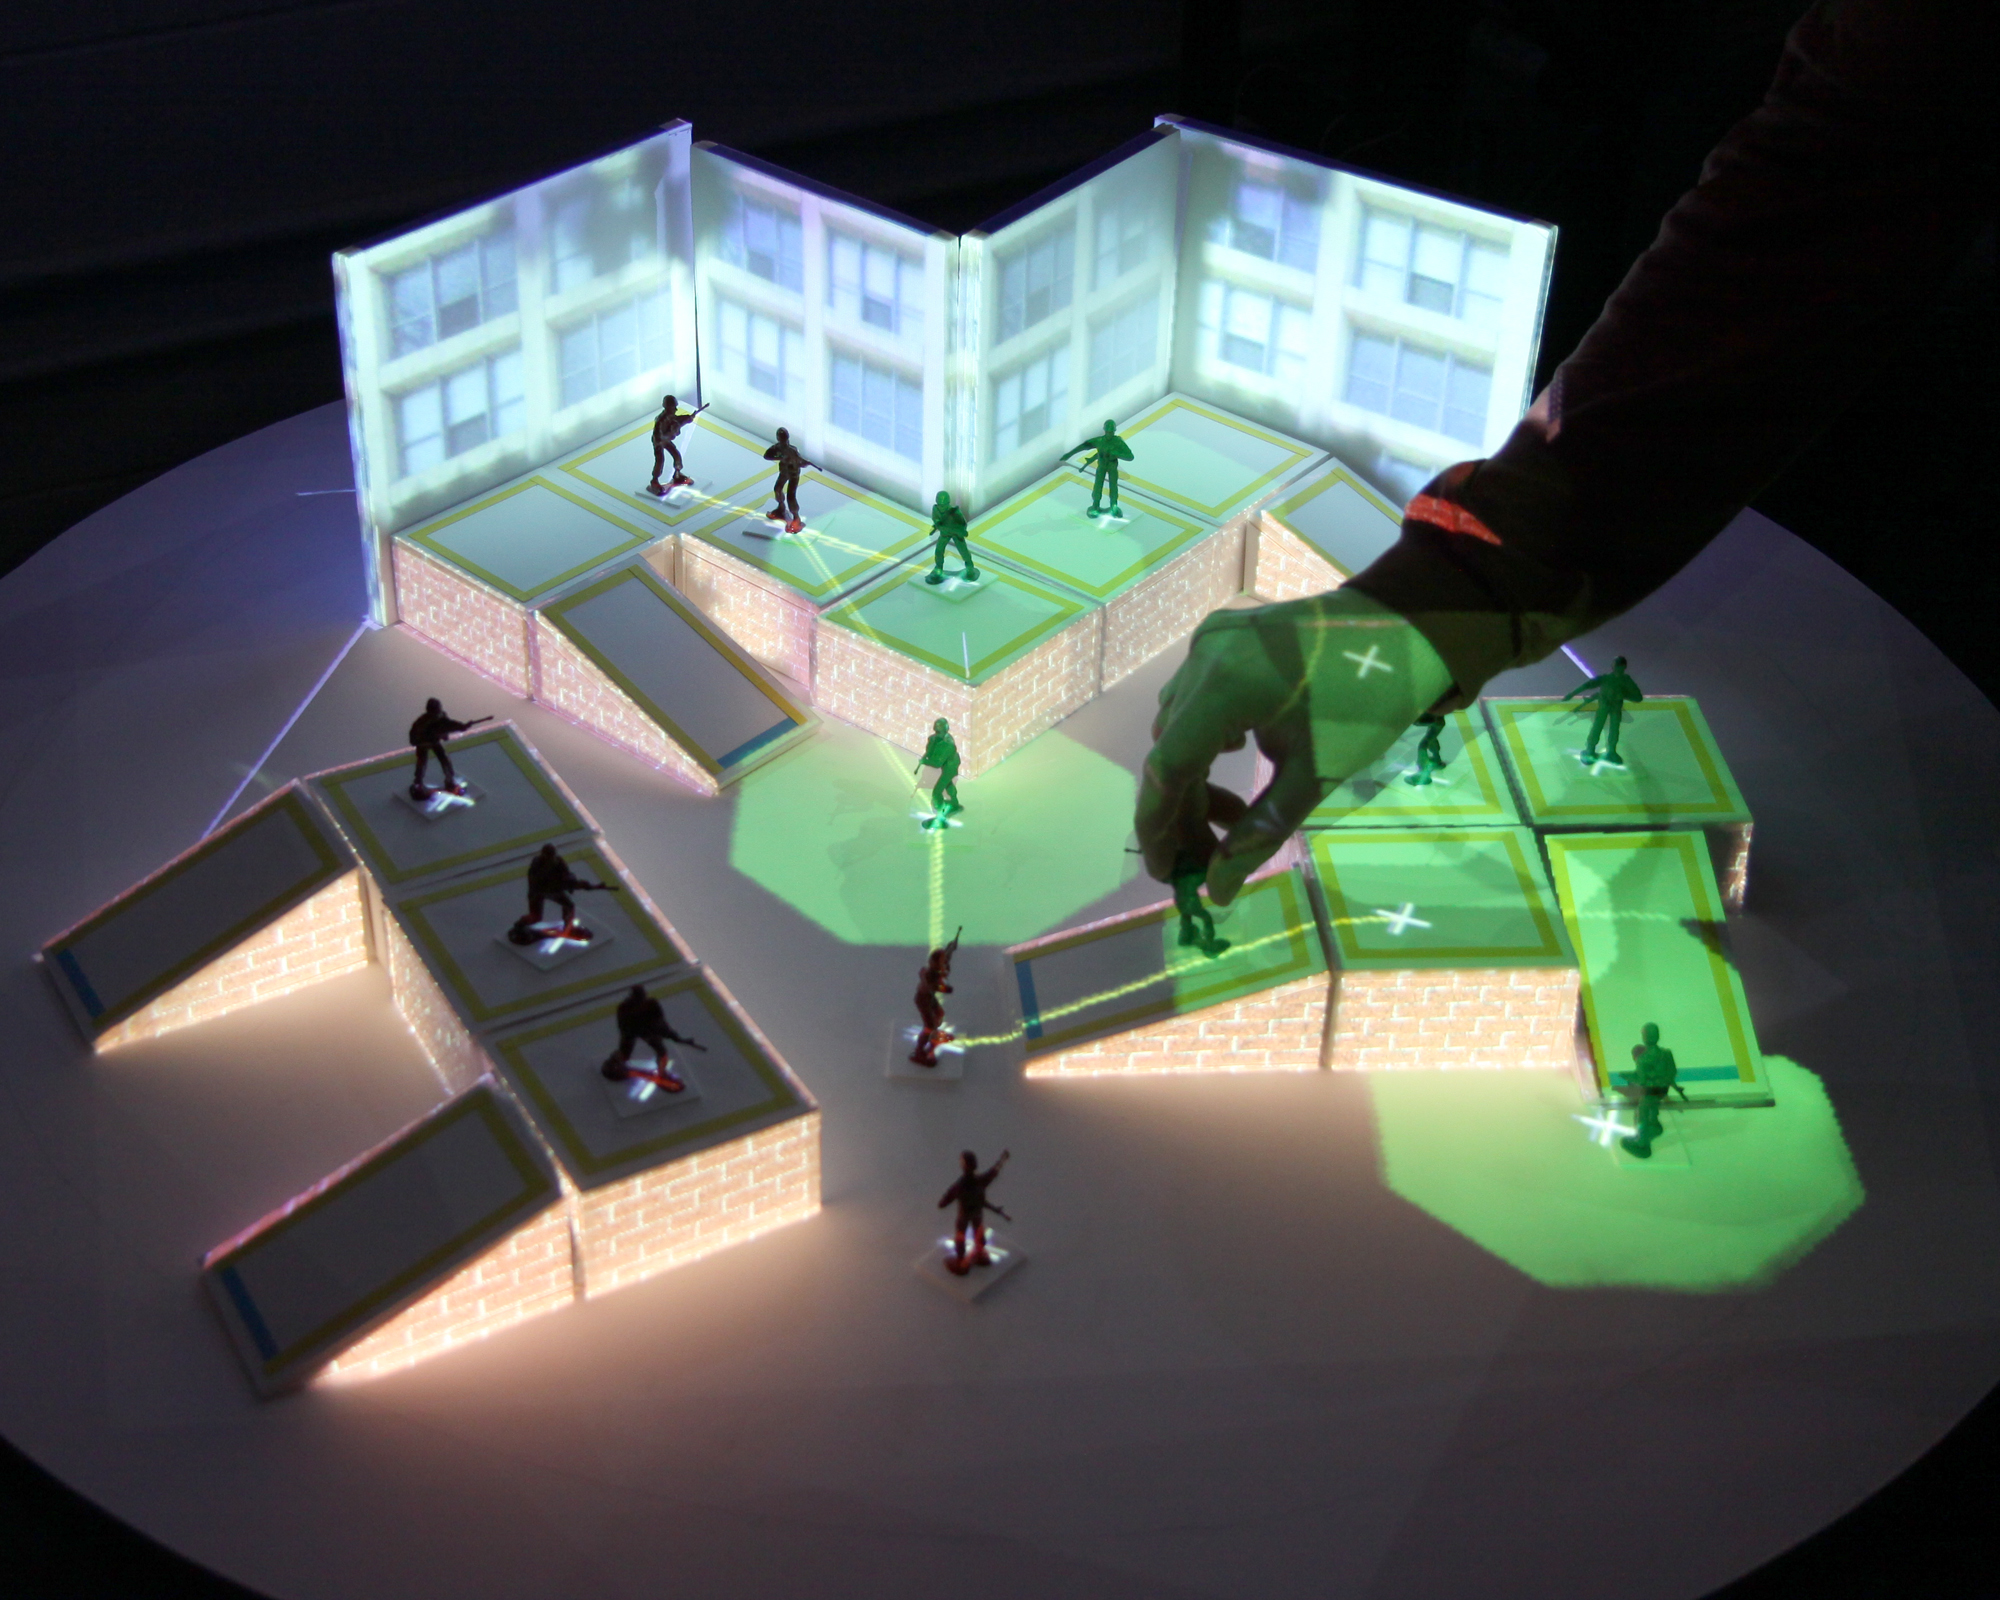
\includegraphics{images/greens_move_3.jpg}}
 \resizebox{\picwidth}{!}{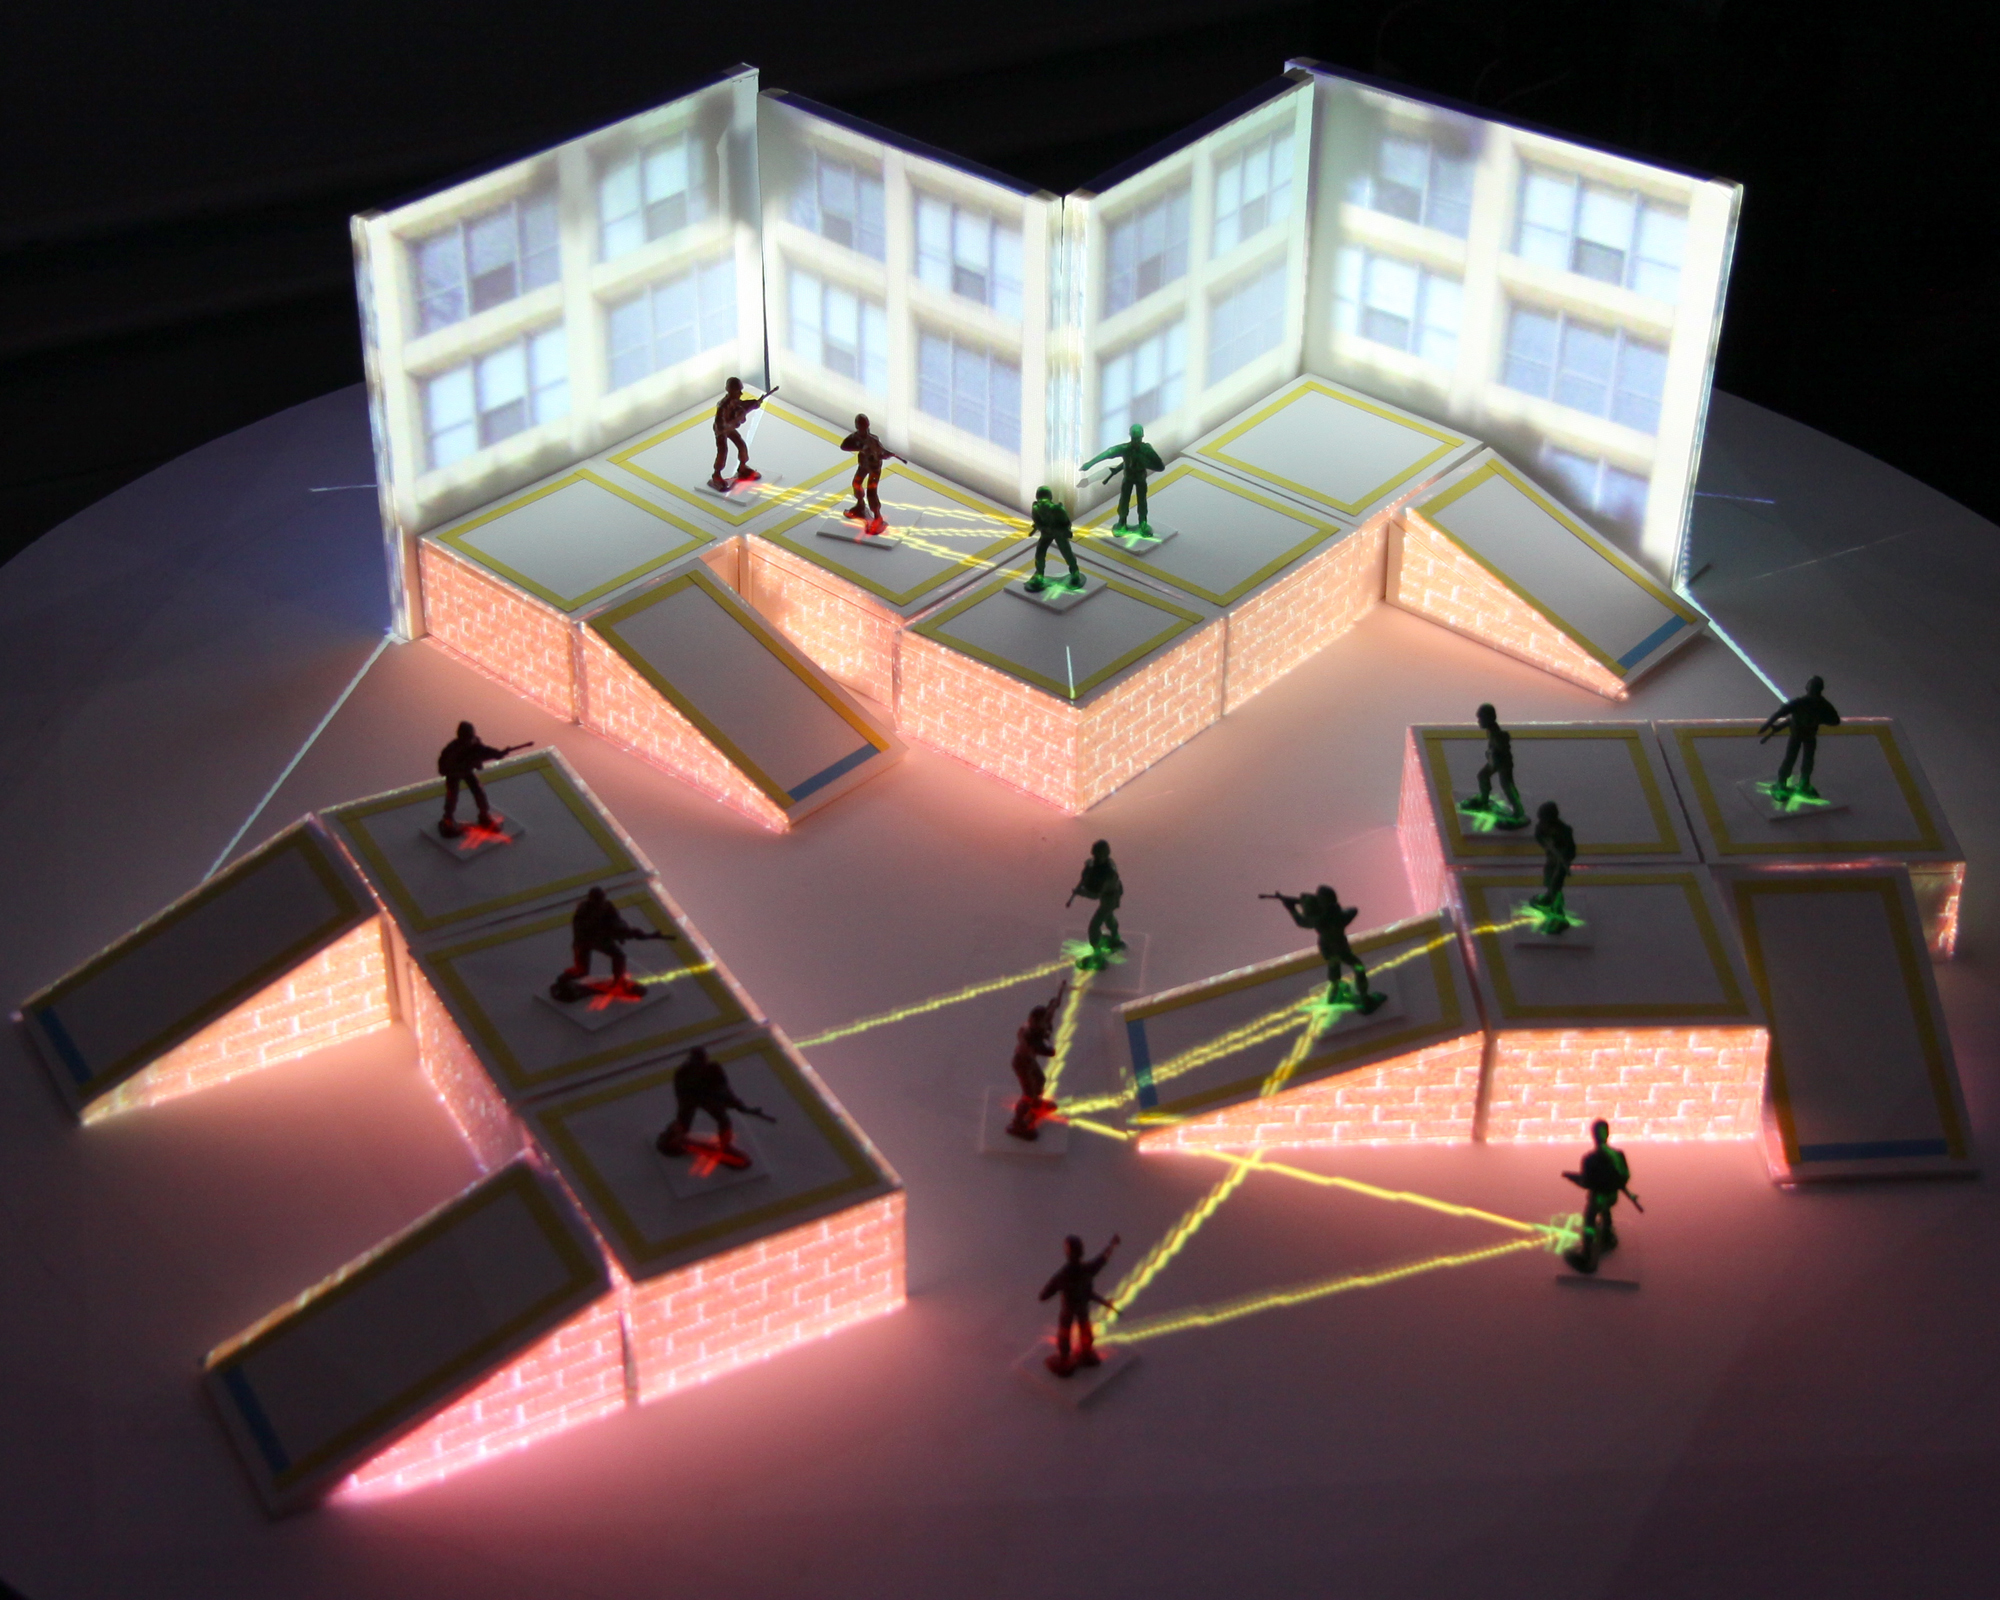
\includegraphics{images/lots_of_combat_2.jpg}}\\
 \resizebox{\picwidth}{!}{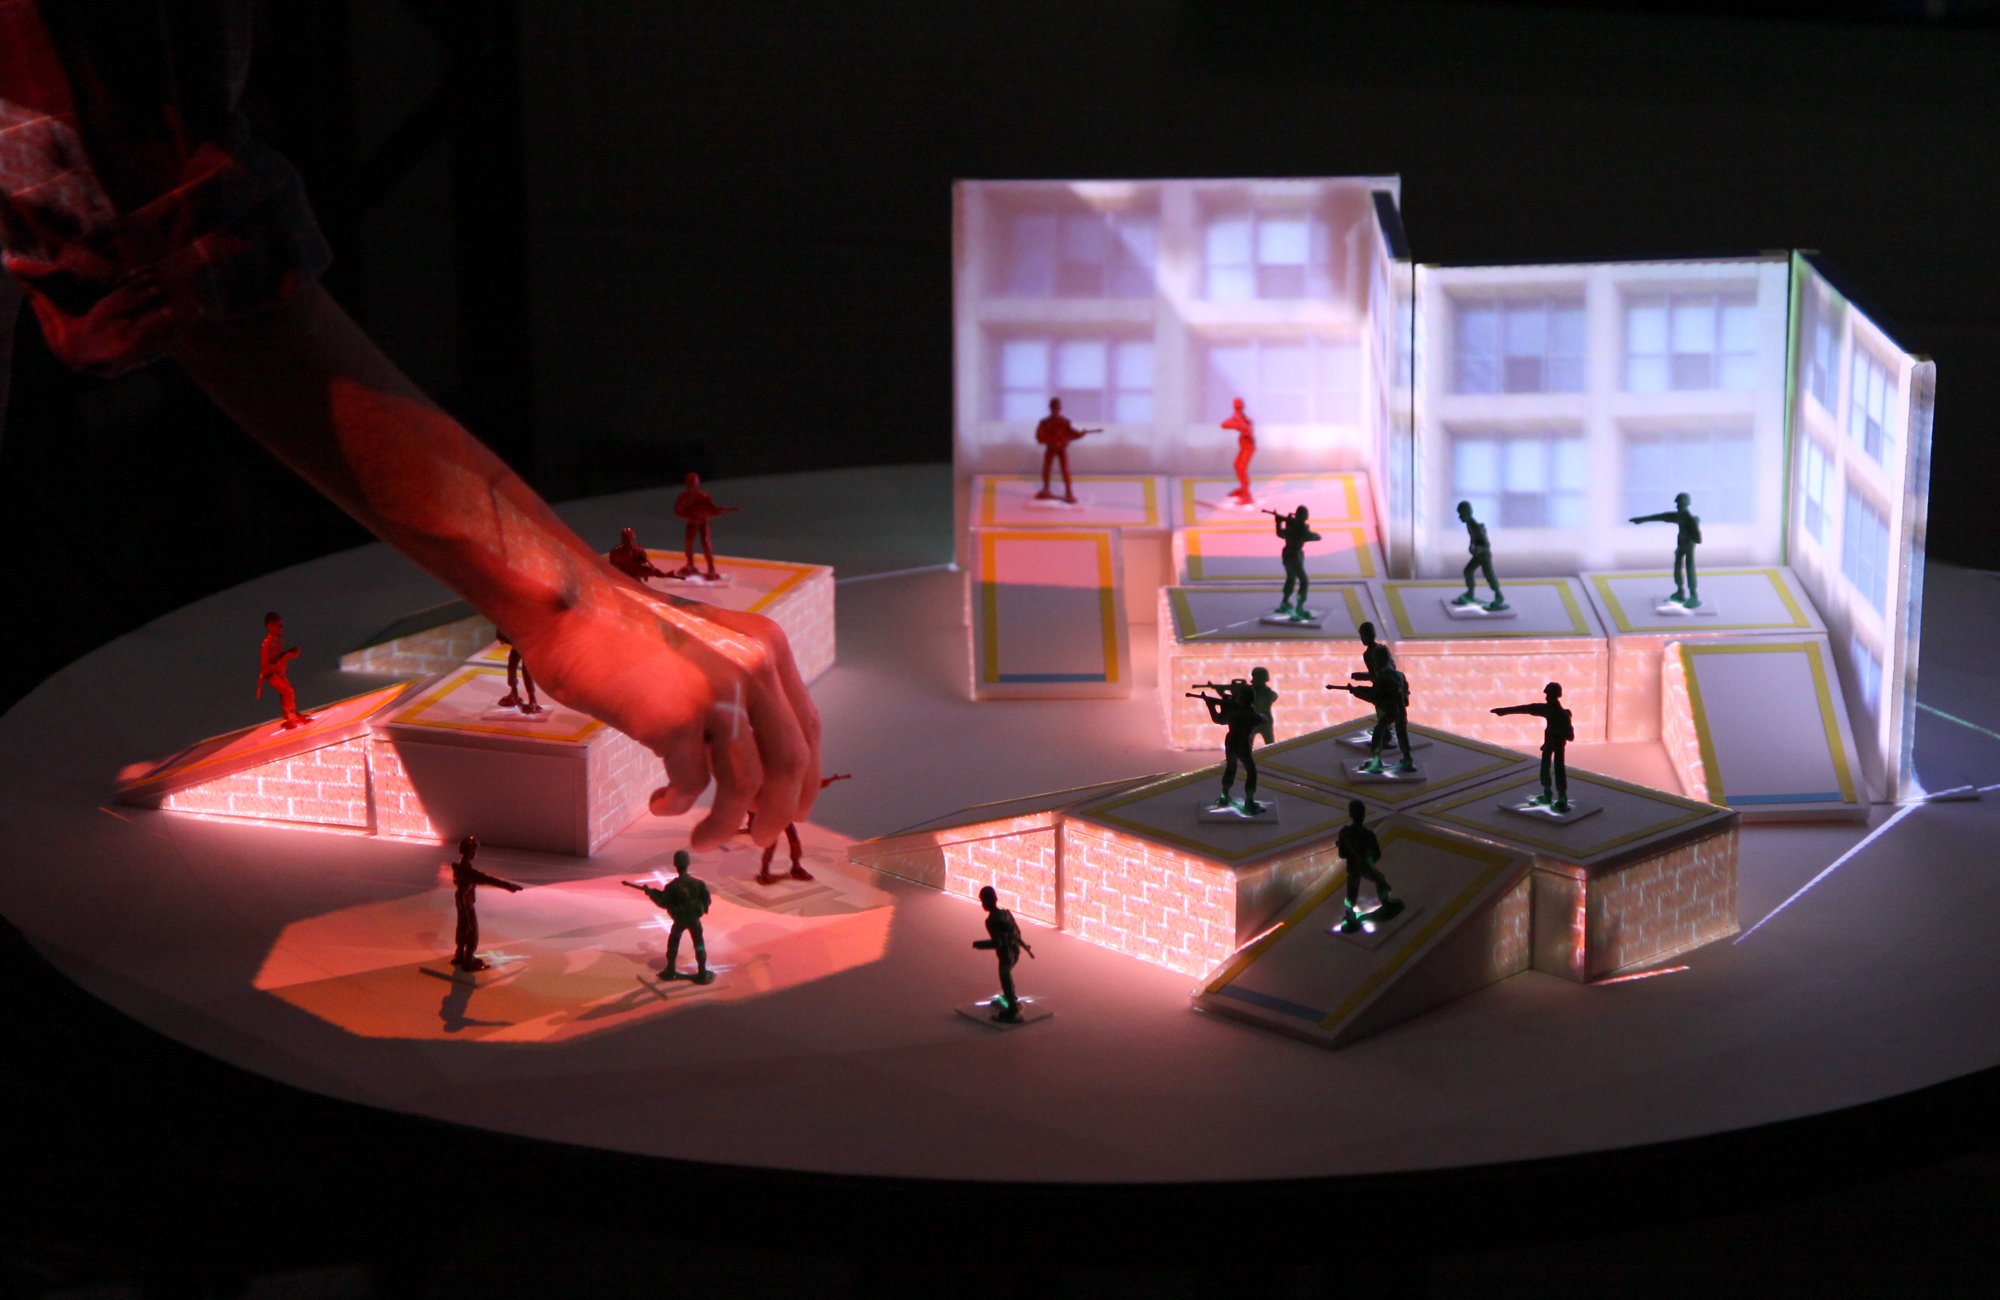
\includegraphics{images/reds_move.jpg}}
 \resizebox{\picwidth}{!}{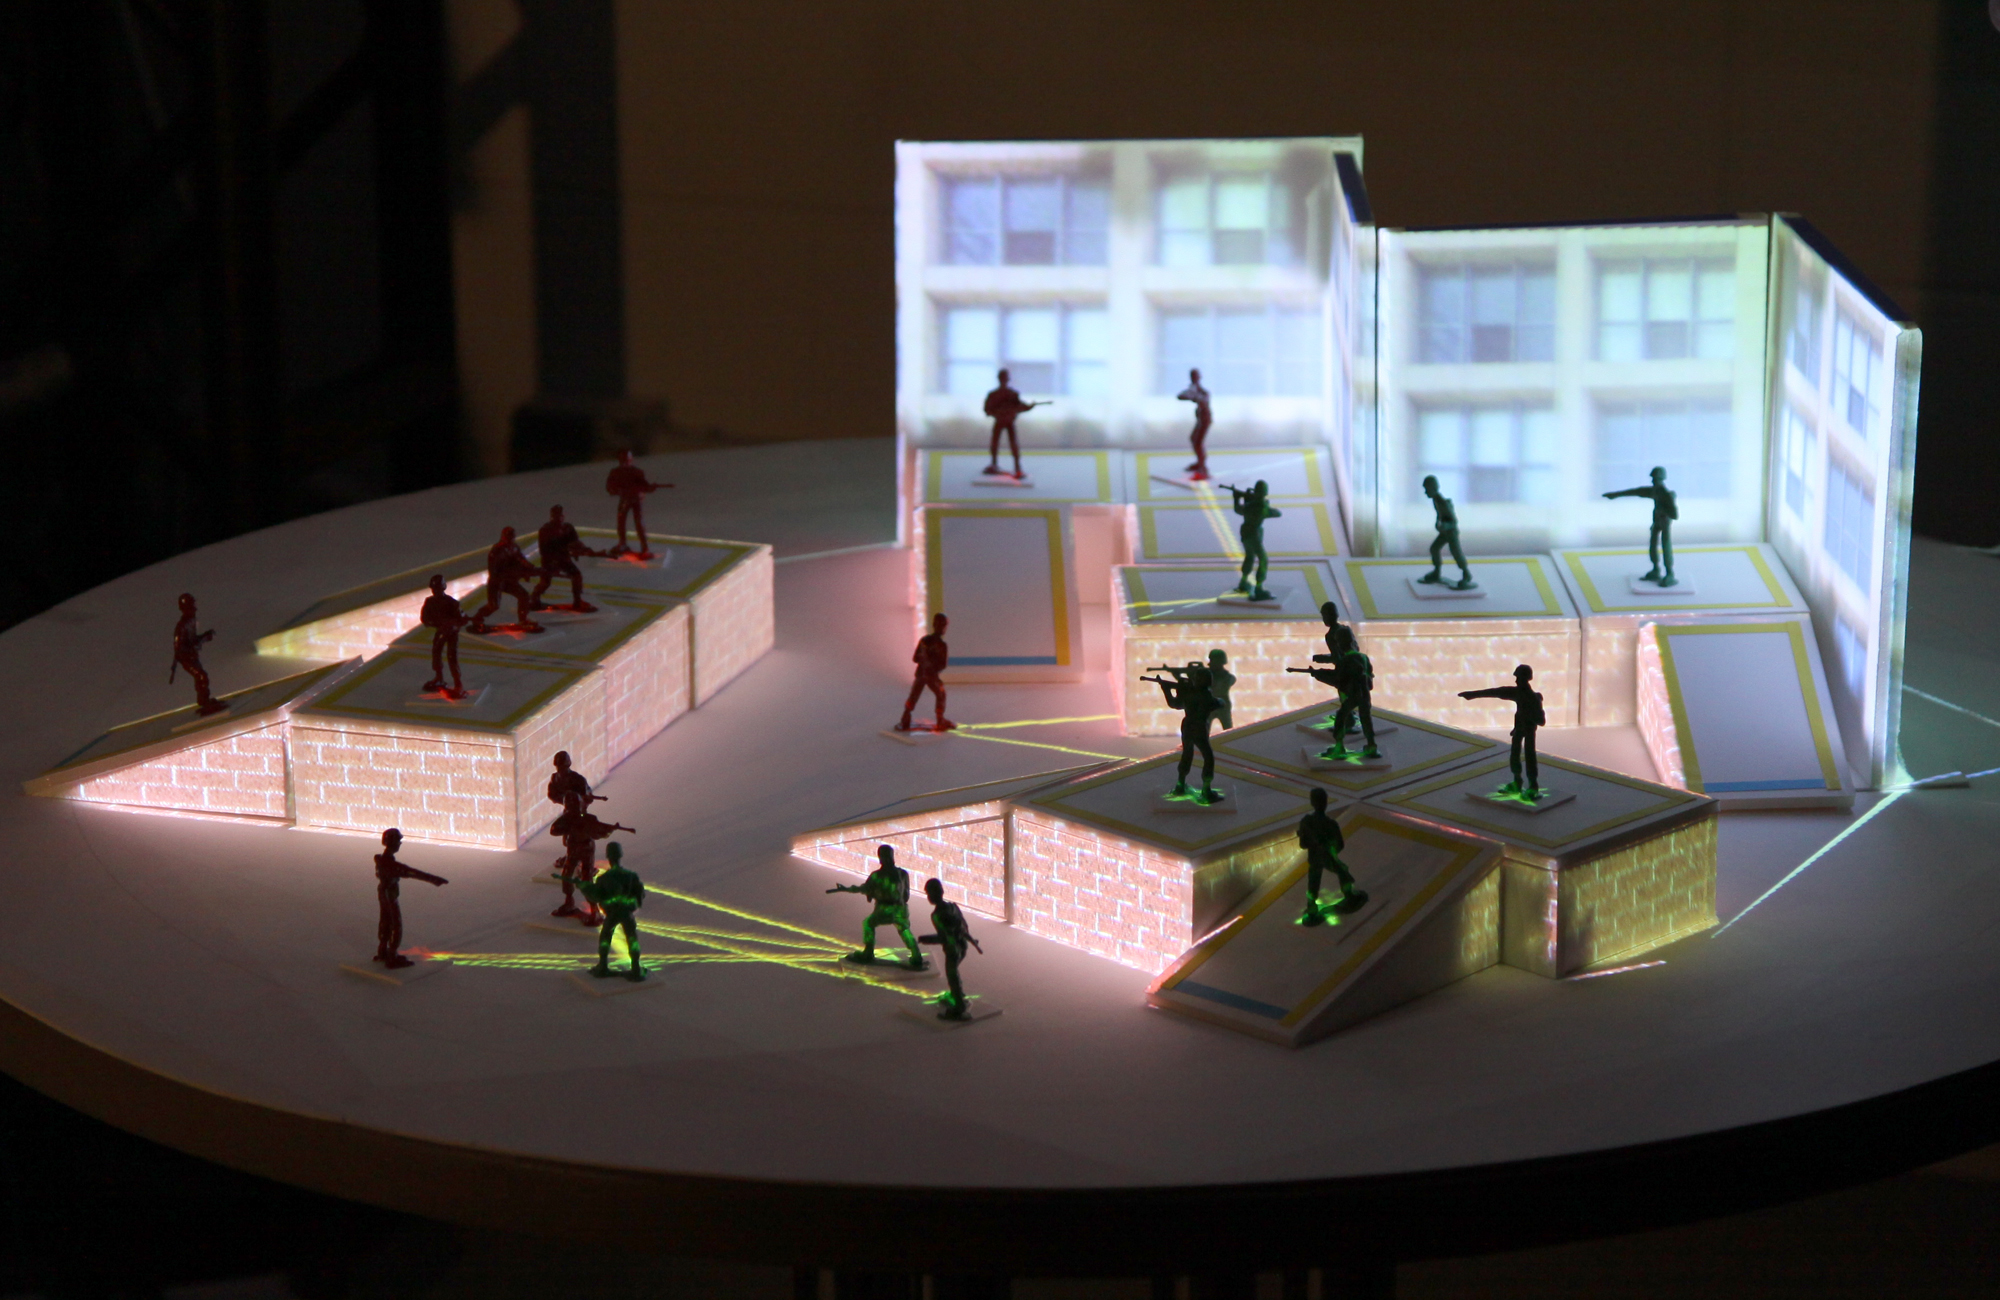
\includegraphics{images/lots_of_combat.jpg}}
\caption[Images of ARmy: A Spatially Augmented Reality Game]{ The above images are snapshots of the \emph{ARmy} application in progress. The application is an example of a spatially augmented reality game, which combines physical game objects with virtual elements through projection. The projections decorate simple, white objects with colorful virtual textures, and display important game information regarding legal moves and simulated combat. }
\label{FIGURE:GameInProgress}
%\vspace{-0.15in}
\end{figure*}

The purpose of this thesis is to summarize my work in developing spatially augmented reality applications to facilitate multi-user game interactions in both small-scale tabletop settings and large-scale immersive environments. In particular, I focus on \emph{ARmy,} a proof-of-concept game prototype that borrows concepts from traditional tabletop war games and augments them with virtual elements, as shown in Figure~\ref{FIGURE:GameInProgress}. I also present a number of applications demonstrating possible ideas for AR games using various devices for interaction in human-scale display environments. Additionally, I describe my contributions to some of the underlying system components that make these applications possible. Finally, I discuss the preliminary results of the applications, as well as aspects that could be expanded through future work.


\chapter{RELATED WORK}

Augmented reality is a relatively recent field, with a large amount of research focusing on how to combine underlying technologies to achieve stable, reproducible systems. Existing work includes a diverse set of techniques, of which spatially augmented reality comprises only a small subset. In order to comprehend the relative advantages and disadvantages of our techniques, it is useful to gain some high level understanding of this broad body of work. The purpose of this chapter is to describe and compare a number of common AR techniques and to provide relevant examples. The discussion focuses in particular on two important problems that must be solved in order to achieve Azuma's definition of augmented reality: the creation of an effective augmented display, and the problem of 3D registration. 

\section{Display Types}

One major component of any AR system is the display technology used to visually integrate the virtual elements with the real world. A wide variety of technologies have been explored by previous research in both augmented and virtual reality, and classifying them can be a challenging task. For the purpose of enumerating some important examples, I adopt the classification scheme of Bimber and Raskar~\cite{BimberBook}, which separates display technologies into three main groups: head-mounted, hand-held, and spatially aligned.

\subsection{Head-mounted Displays}

Head-mounted displays (HMDs) comprise the earliest and most dominant display technology used in augmented reality applications. As their name implies, head-mounted displays are devices physically worn by the user, generally composed of some eye-aligned viewing equipment that provides the augmented visuals. The earliest and most typical HMDs can be classified as optical or video-based see-through displays, although more recent research has also explored head-mounted projectors, %~\cite{Kijima1997}
%~\cite{Parsons1998}
%~\cite{Inami2000}
%~\cite{Hua2001}  
and retinal display methods.
%~\cite{Kollin1993}~\cite{Pryor1998}~\cite{Lewis2004}.

The first head-mounted display, and therefore the earliest example of augmented reality, is credited to Ivan E. Sutherland ~\cite{Sutherland1968}, who developed an optical see-through display to present the viewer with perspective images of three-dimensional, virtual, wireframe objects. An optical see-through display is one in which the user looks through an optical combiner, such as a partially transparent mirror. The combiner allows some light to pass through while simultaneously reflecting computer-generated images into the viewer's eyes, thus combining real and virtual images. In contrast, a video-based augmented display provides a view of the physical world through video footage. Images are captured via camera and combined in real time with computer-generated visuals before being displayed on some form of head-mounted monitor. Numerous survey papers exist which compare and contrast optical and video-based HMDs~\cite{Rolland1994, Azuma1997}.

In general, head-mounted displays are cited as being good candidates for portable AR applications in that they equip users with personal display devices that could be worn in a variety of settings. However, they also suffer from a number of disadvantages. Because HMDs typically rely on small, eye-aligned displays, they tend to be limited in both display resolution and field of view. Bimber and Raskar note that the hardware required for many head-mounted devices may be expensive to construct, difficult to properly calibrate, and at times too heavy for users to wear comfortably~\cite{BimberBook}.

\subsection{Hand-held Displays}

In contrast to head-mounted displays, hand-held displays are those in which the display technology is embedded in small, portable, hand-held devices. Generally, hand-held AR systems aim to use the portable devices already available to the average consumer today, including cell phones, personal digital assistants (PDAs), and laptop PCs. Such devices already contain small monitor or touch-screen displays, as well as digital cameras, which make them viable candidates for video-based see-through AR techniques. Most importantly, these devices represent technology that has already become ubiquitous, providing an immediate platform for AR applications for everyday use.

A potential limitation of hand-held AR applications is that many mobile devices lack the computational power and resources of larger systems. One solution is to develop applications as lightweight clients that offload heavy computations onto remote servers, such as in the work of Pasman and Woodward~\cite{Pasman2003}, who developed a client/server framework for AR applications on a PDA using data compression schemes for fast network traffic. Wagner and Schmalsteig~\cite{Wagner2003} presented an AR implementation for an off-the-shelf PDA capable of running in both a self-contained stand-alone mode and a distributed networked mode. Their system switches between the two methods dynamically to adapt to variable network availability.
%~\cite{Geiger2001} 
%~\cite{Gausemeier2003} 
%~\cite{Pasman2003}~\cite{Wagner2003}.

Hand-held AR techniques are beginning to find prominence within the video game industry. Perhaps the most notable example is the Nintendo 3DS, a hand-held video game system equipped with multiple cameras and an autostereoscopic screen, allowing for video see-through techniques to be combined with 3D effects~\cite{Nintendo3DS}. The system comes with a library of AR games, which can be played by aiming the camera at a set of provided marker cards. A similar example is \emph{ARhrrrr!}, an AR game developed by Georgia Tech Augmented Environments Lab and the Savannah College of Art and Design, which also uses a mobile device as a video see-through display~\cite{ARhrrrr!}. The game overlays graphics onto a physical paper map, and also incorporates other tangible objects, such as brightly colored candies.

\subsection{Spatially Aligned Displays}

The third and final category of AR display devices is characterized by displays that are completely unattached to the user, but instead consist of fixtures physically aligned with the environment. These \emph{spatially augmented reality} (SAR) techniques represent the particular branch of AR under which our current research falls. Some spatial displays apply optical or video-based see-through techniques by using stationary screens or monitors to display the augmented visuals. For example, Bimber et al. present a ``Virtual Showcase,'' which uses half-silvered mirror combiners to create an enclosed AR display analogous to the physical showcases typical of museum exhibits~\cite{Bimber2005}. However, the spatial display techniques most related to our research are those which employ direct augmentation, typically by displaying virtual information directly on the surfaces of physical objects using some configuration of video projectors.

An important and well-known example of projector-based spatial display techniques is the CAVE (CAVE Automatic Virtual Environment) system developed by Cruz-Neira et. al~\cite{Cruz-Neira1993}. Although the CAVE is technically classified as an example of virtual reality, it stands as a significant precursor to SAR techniques. The display area is an enclosed room comprised of rear-projection screens and a top-down projector for displaying images on the floor, thus allowing for an effective immersive environment. The user is equipped with head-tracking devices and 3D goggles for stereoscopic image display.

Raskar and colleagues have presented the ``Office of the Future,'' which explores the possibility of using SAR applications in the setting of an everyday workspace to facilitate telepresence and computing tasks~\cite{Raskar1998a}. They proposed using multiple projectors to present images on irregular, nonplanar surfaces, and demonstrated a technique for generating images suitable for such displays~\cite{Raskar1998b}. Their later work expands upon these techniques with the idea of ``Shader Lamps'', which allow for augmentation of complex 3D objects to create the appearance of desired material properties, such as color and texture~\cite{Raskar2000}. 

A significant underlying theme of much projection-based SAR research is the vision of a future in which these display technologies have become truly ubiquitous. Underkoffler et al. presented the idea of a ``Luminous Room,'' lit by multiple ``IO bulbs,'' which combine a projector and camera to facilitate both spatial display and user interactions~\cite{Underkoffler1999}. Pinhanez proposed the use of ``Everywhere Display'' projectors equipped with poseable mirrors that allow for the projection to be steered to any suitable surface within the surrounding environment~\cite{Pinhanez2001}. The idea behind each of these techniques is to create a compact SAR device that can be reasonably reproduced and distributed for use in homes, workplaces, schools, commercial venues, and other public settings.

Spatially augmented reality techniques offer a number of advantages over user-attached display technologies. One benefit is that SAR displays are capable of covering large surfaces in full-scale, immersive environments, and therefore provide higher resolution displays with a wider field of view. With the exception of specific view-dependent effects, general augmentation of a scene can be experienced by any number of users independent of the number of display devices. Therefore, achieving a shared multi-user environment may be easier with SAR than with head-mounted or hand-held methods, which require that each user be equipped with a personal display device. Because spatial displays generally do not require such devices, users are able to experience a higher degree of mobility and comfort while participating. Yet another advantage is that when properly calibrated, spatial display devices do not suffer from as many visual disparities as see-through displays, which may produce large amounts of error in cases of misalignment. For example, projector displays can more easily create realistic looking augmentation because the virtual elements are directly applied to real objects, which have physical presence in the scene free from spatial inconsistencies.

Despite these benefits, spatially augmented reality does entail a number of drawbacks. Direct projector-based methods are capable of augmenting the physical surfaces in the scene, but are generally unable to display virtual objects with volume. In other words, three-dimensional objects cannot be created from thin air, but must have a physical basis in the real scene. Another issue is that although SAR display configurations are becoming cheaper and easier to produce, at present these systems are not as ubiquitous as hand-held devices. Therefore, while current SAR environments may be good candidates for fixed locations, such as museum exhibits, conference rooms, or amusement park rides, they do not yet offer immediate solutions for mobile AR applications.

Our previous research has focused on visualization using direct augmentation through multi-projector, multi-surface systems. One application that we have explored with this system is an architectural daylighting design tool, which allows the user to design a physical room using movable projection surfaces as walls. We then use multiple projectors to display simulated lighting and material properties on the physical room model, creating a virtual heliodon that allows the user to observe different designs under natural lighting conditions for any given time and day of the year. We have experimented with this technology in a tabletop setting with miniature models, as well as in a large-scale, immersive setting with full-scale walls~\cite{Sheng2009, Yapo2010}.

% FIGURE OF CONTRAPTION RIG (DIAGRAM AND PHOTO)

\begin{figure*}[t]
\newcommand{\picheight}{3in}
 \resizebox{!}{\picheight}{\includegraphics{images/new_contraption.png}}
 \resizebox{!}{\picheight}{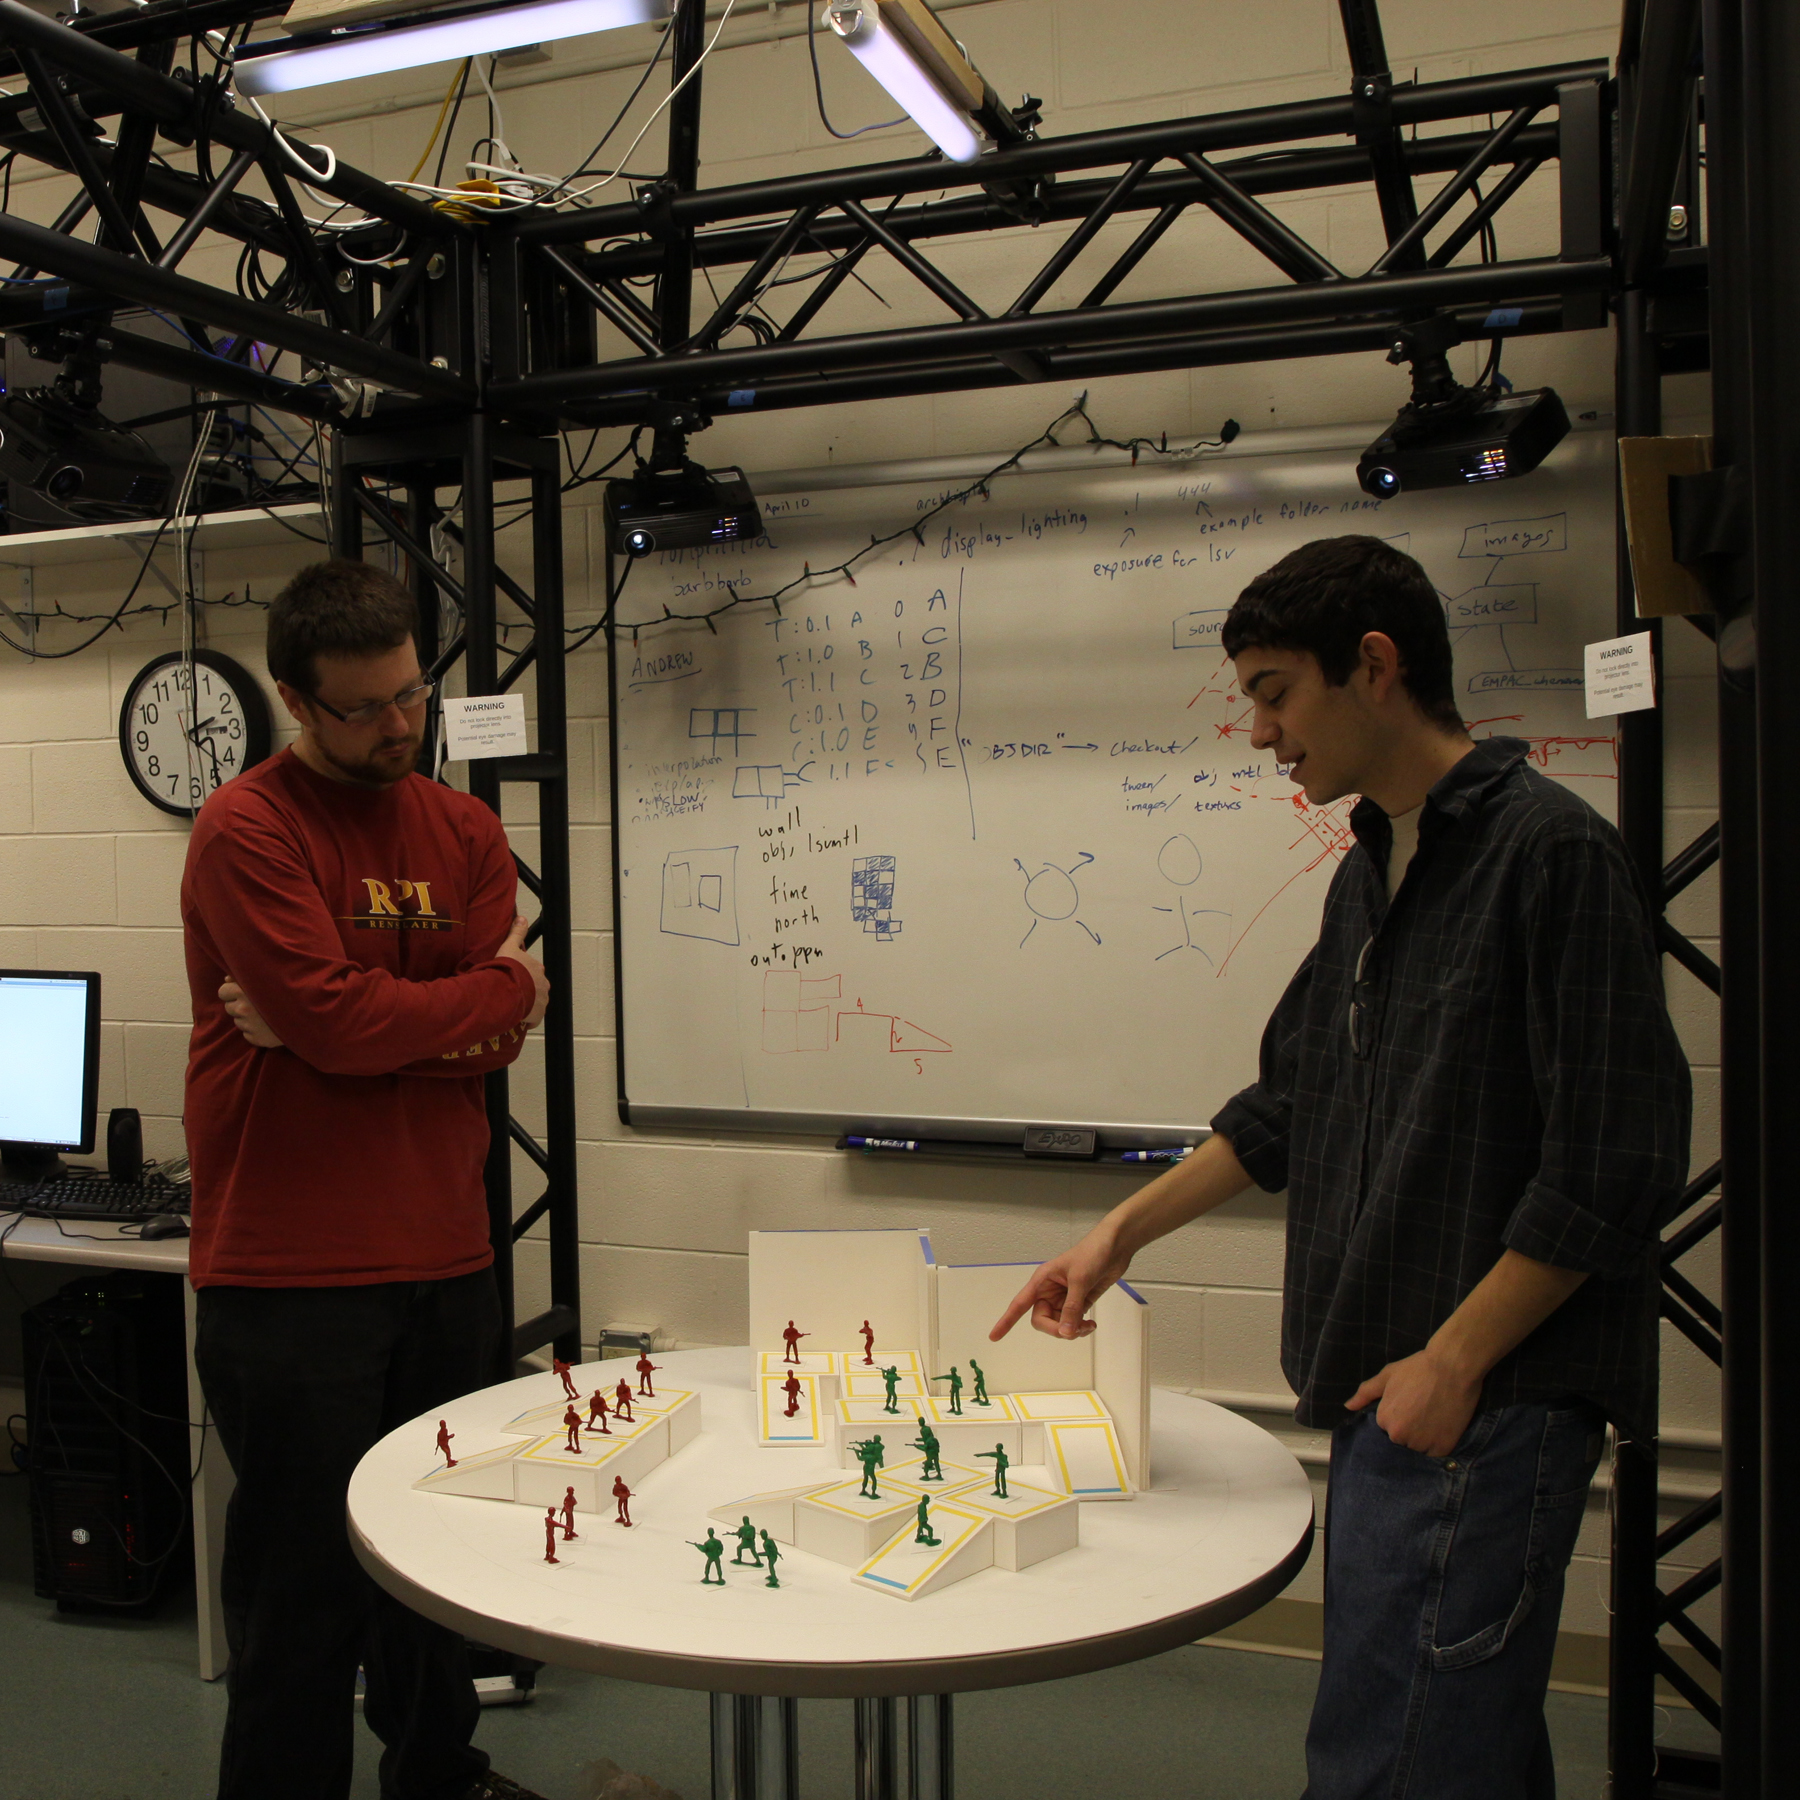
\includegraphics{images/contraption_with_people.jpg}}
\caption[Projector/Camera Rig]{Our spatially augmented reality rig is equipped with a single camera for object detection and multiple projectors for display. It is designed to fully cover the surface of a centered table, which acts as a space for user interactions. }
\label{FIGURE:contraption_rig}
\vspace{-0.15in}
\end{figure*}

\section{3D Registration}

In addition to displaying virtual objects within the real world, augmented reality ideally allows the user to interact with the virtual elements in an intuitive way. In order to provide convincing visuals and a means for interaction, the virtual objects and display devices must be registered in 3D relative to the physical environment. Generally this involves two main steps: calibration and tracking.

\subsection{Calibration}

Calibration refers to the problem of correctly modeling and recovering geometric correspondences between display or tracking devices and the physical environment. In the case of projector-based displays, it is necessary that we be able to map each projector pixel to a known point relative to the world coordinate system so that we can use that information to project images that are correctly aligned with the physical display surfaces. In addition, since camera devices are required for vision-based techniques used in the tracking step, these devices must also be calibrated.

Camera calibration is a classical vision topic that has been researched thoroughly. Typically cameras and projectors are described using the pinhole model, which maps 3D points in the world to 2D image coordinates using both intrinsic parameters, which describe center, scale, and skewness of the image coordinate system, and extrinsic parameters, which describe the rotation and translation of the camera relative to world coordinates. Zhang~\cite{Zhang2000} provides a simple, robust method for calibration in which the user captures multiple images of a single, planar calibration target from differing points of view. The method requires no a priori knowledge of the position, orientation, or movement of the target relative to the camera. Additional research has focused on recovering calibration parameters even in cases involving significant lens distortion. For example, Scaramuzza et al.~\cite{Scaramuzza2006} provide an effective means for calibrating omnidirectional cameras, as well as cameras equipped with a fisheye lens.

\subsection{Tracking}

Once the display and vision devices are properly calibrated within the world coordinate system, we can use them to accomplish tracking of physical objects for augmentation. Unlike calibration routines, which typically are done once during setup, and therefore can accommodate somewhat time-consuming, manual tasks, tracking must be done automatically and efficiently at interactive rates for the system to be responsive. Effective registration has been achieved by utilizing electromagnetic and mechanical tracking devices, such as in the CAVE system~\cite{Cruz-Neira1993}, as well as vision-based techniques, which are discussed below.

\subsubsection{Fiducial Markers}

A large variety of AR applications use fiducial markers to identify objects and determine their position and orientation. Kato and Billinghurst~\cite{Kato1999} provide a method for tracking square, planar markers with a black border and bi-tonal interior pattern. Their method identifies markers in the camera image by using edge-based vision techniques to detect quadrilaterals. Detected regions are normalized, sampled, and compared via correlation to a set of marker patterns provided a priori by the user. They present their technique in the context of an augmented reality conferencing system, and have released a working library known as the ARToolkit, which has since become well-known and widely used within the AR community. Using a similar quadrilateral-based method, Fiala~\cite{Fiala2005} employs digital processing techniques to identify square markers bearing ten-digit identification codes, encoded in the form of six-by-six bitonal grids similar to barcodes. This tracking system, known as ARTag, provides the user with a large library of predefined markers, and leverages redundancies in the encoding technique to identify markers even under conditions of partial occlusion.

Fiducial marker systems hold great promise for AR game applications, as they provide a viable, inexpensive means of identifying specific game-related objects. For example, markers could be printed on cards, attached to wooden game pieces, or positioned at the corners of a movable game board in a manner similar to the augmented whiteboard used in Kato and Billinghurst's conferencing system~\cite{Kato1999}. 
One disadvantage of fiducial markers is that the robustness and accuracy of the tracking generally depends on the relative size of the markers in the camera image, since an image of a marker that is too small or far away may not yield sufficient resolution for the tracking algorithm to identify the contained pattern. Thus, suitable tracking may require markers that are too large or unwieldy for players to use comfortably. In addition, large fiducial markers may interfere with the visual quality of virtual elements projected onto them. This presents an added problem for projector-based SAR systems, which, unlike see-through AR displays, cannot fully hide the marker with rendered objects.

\subsubsection{Structured Light}

Other useful methods for 3D registration employ structured light techniques, which project known pixel patterns into the scene and measure the result in order to recover depth information. Ashdown et al.~\cite{Ashdown2004} use a variation of structured light to project successive patterns containing continuous horizontal and vertical lines. The method detects ``kinks'' in the lines and uses this information to segment the image into multiple planar regions, which are then stitched together into a continuous display by refining their individual homographies to fit adjacency constraints. Lee et al.~\cite{Lee2004} propose a structured light method for registering projection surfaces without the use of a camera and vision techniques. Instead, the corners of the target surface are embedded with light sensors, which detect and transmit the binary sequences projected in the patterns. The system uses this information to identify the quadrilateral region of the surface within the projector image and warps images accordingly. 

\subsubsection{Imperceptible Pattern Embedding}

A potentially serious hurdle for the application of fiducial marker and structured light techniques to display systems that use direct augmentation is interference from projected images. In other words, projecting a colored image onto a surface bearing a fiducial marker may obscure the pattern of the marker in such a way as to prevent correct identification by the tracking algorithm. Projected structured light patterns suffer from the same problem, and may obstruct the displayed images or otherwise distract the user. 

One possible solution to this problem involves directly embedding structured light patterns into the display images in such a way as to remain imperceptible to the user. Lee et al.~\cite{Lee2005} demonstrate an improvement on their previous sensor-based technique which is able to embed the light patterns into perceptually uniform gray blocks, which are less distracting than high-contrast patterns. Although the method is shown to achieve accurate tracking at interactive framerates, regions bearing the embedded patterns are still visible to the user and reduce the overall display space available for application content. In addition, the method is shown to work only with a modified projector that outputs grayscale images.

Cotting et al.~\cite{Cotting2004} propose a method that achieves direct pattern embedding by taking advantage of unmodified DLP projectors, which use precisely-timed modulation of micro-mirrors to determine the intensity and color of each image pixel. Each pixel corresponds to a single mirror, which switches between a ``white'' position that tilts toward the projector light source, thus contributing high intensity light to the image, and a ``black'' position that tilts away, thus contributing little light. Their method first measures the sequences of mirror flips across the full range of color values for each independent color channel. Then it remaps each pixel to a perceptually similar color value such, that during a predetermined exposure time, the mirror's position matches the specified black or white value of the desired light pattern. Using carefully calibrated exposures, the camera can acquire images of the light pattern without greatly degrading the image quality of the simultaneous display. Although appealing, short-exposure methods such as this require the extra work of precisely synchronizing the camera and projectors.

\subsubsection{Infrared Tracking}

Another solution to the problem of simultaneous acquisition and display is to track objects based only on specific wavelengths of light which are not projected in significant amounts by the display. A significant amount of research has experimented with tracking using infrared light, which is invisible to the human eye and therefore does not interfere with displayed images. For example, Lee et al.~\cite{Lee2007} have presented the use of a hybrid LED projector capable of transmitting both infrared and visible light in order to simultaneously display visible application images and invisible structured light patterns. Although an excellent proof of concept, the proposed method does not work with standard commodity projectors.

More recent work has led to the development of commercially available 3D range cameras, which use infrared structured light techniques to produce real-time depth images of a measured scene. Perhaps the most widely known example of this kind of registration is Microsoft's Kinect, a recent Xbox 360 peripheral that uses a depth-image camera as an input device for motion-based controls~\cite{Kinect, Shotton2011}.

A different approach to infrared-based tracking is to use more conventional infrared-emitting devices, such as LED markers or laser pens. Kato and Billinghurst demonstrated the use of an infrared LED-tipped stylus that allowed users to interact with a virtual whiteboard~\cite{Kato1999}. The LED activates in response to pressure on the tip of the stylus, and is detected by a calibrated infrared camera. Because the surface location of the whiteboard is known, the system is able to determine the location of the pen tip in screen coordinates, allowing the user to write or draw on the augmented display.

\subsubsection{Color-based Tracking}

Color information provides another potential means for detecting and registering objects. For example, the Luminous Room project presented by Underkoffler et al.~\cite{Underkoffler1999} used a simple tagging system through which application-specific objects were marked with small groupings of colored dots. The system identifies objects by first detecting dots as regions of specified size and color, and then by grouping individual dots based on patterns with known distance and angle constraints. An advantage of color-based techniques is that they are generally simpler to implement and at times faster than more sophisticated vision algorithms. 

One problem of color-based techniques is that they may not be highly robust under inconsistent lighting conditions, and are likely to suffer from a high number of false positives, as target colors may appear within background clutter. The Luminous Room prototype avoids these problems by using special reflective dot markers which appear brighter in the camera image, allowing them to be easily separated from the background. In addition, colored markers share the same problem as bitonal fiducial markers, in that projected visuals are likely to obscure the appearance of the marker, making it difficult to achieve simultaneous capture and display. Despite these drawbacks, color-based object recognition may be useful in the context of SAR games, since color is commonly used in games to distinguish objects that appear otherwise identical. Thus it might be possible to track specific game pieces without the need for added markers.

\subsubsection{Human Tracking}

In addition to tracking physical game pieces, another set of interactions can be achieved through the tracking of the users. 
For example, the Kinect tracks the user's body and maps it to a skeleton model in real time, allowing for game applications to use full-body gestural controls~\cite{Shotton2011, Kinect}. Other research has tried to achieve accurate tracking of specific body parts, most commonly focusing on the human hand. Lee and H\"{o}llerer present Handy AR, a system for markerless tracking that detects and estimates the 3D pose of an out-stretched human hand~\cite{LeeT2007}. This provides the benefit of allowing the user's hand to act in place of a fiducial marker, but requires the hand to remain out-stretched during use. More recently, Wang and Popovi\'c~\cite{Wang2009} have proposed using a lightweight colored glove to allow for more robust detection of a wide variety of hand poses, including such complex gestures as the alphabet used in American Sign Language.

\section{Summary}

The blending of real and virtual entities through augmented reality has been the focus of a wide range of research, combining contributions from engineering, graphics, and computer vision. Augmented reality requires the use of specialized displays, which have been implemented in various ways, including the use of head-mounted, hand-held, and spatially aligned devices. In addition, consistently aligning virtual elements with the physical scene typically requires accurate 3D registration of physical objects, which has been achieved using electromagnetic devices, structured light patterns, fiducial markers, and infrared-based or color-based tracking.

\chapter{SAR GAME APPLICATIONS}
% or \chapter{SPATIALLY AUGMENTED REALITY GAME APPLICATIONS} ?

In this chapter, I will present a number of interesting prototype applications designed to demonstrate the capabilities of our developing system and to explore possible uses of SAR techniques. I will describe the basic design of each application and the user interactions that they facilitate. A more detailed discussion of the underlying implementation is presented in the next chapter.

\section{ARmy Simulation Overview}

The ARmy application is a military simulation game played between two opponents. The game is in many ways similar to a typical tabletop war game, in that it uses miniature objects to create a physical representation of the game world. The players are given a number of plastic soldier figurines, referred to as \emph{units}, which represent their respective armies. Each player moves his units through the scene according to the rules of the game, engaging in combat with opposing units to eliminate them from play. Victory is achieved by completely eliminating the opposing army.

Most tabletop games are played over a number of turns consisting of multiple steps, through which the players progress at their own pace. In the same way, the ARmy application is designed as a series of player-controlled feedback loops, meaning that the game module only proceeds at the request of the players. The current implementation relies on a simple wireless remote control, which allows the players to send two different signals to the game module. The first is an ``update request,'' which tells the game to update its model of the scene and display any new information. The second is a ``continue'' command, which indicates that the players have finished with the current stage of play and wish to proceed to the next step. Figure~\ref{FIGURE:ARmyDiagram} diagrams the overall design of the interaction using a finite state representation.

\begin{figure}[p]
\begin{center}
\includegraphics[width=5in]{images/game_diagram.pdf}
\end{center}
\caption[ARmy Application State Diagram]{\small{State diagram of the ARmy application. Gray boxes represent stages of play defined by player actions. Blue boxes represent stages performed completely by the game module. Similarly, black arrows represent transitions triggered by the players via the remote control, while blue arrows represent automatic transitions.}}
\label{FIGURE:ARmyDiagram}
%\vspace*{-0.15in}
\end{figure}

In designing this application, special consideration was given as to how SAR techniques could be leveraged to improve upon the play style of traditional tabletop games. This section provides a step-by-step description of how the game is played, as well as how it incorporates virtual elements to create a new and interesting game experience.

\subsection{Terrain Placement}

An important aspect of many tabletop games, particularly those that involve military strategy, is the idea that the game world is not flat and uniform, but rather that it is characterized by varying terrain. As in the real world, terrain represents variations in elevation and environment that affect units within the area. For example, one kind of terrain might represent a swamp that is difficult to walk through, resulting in a movement penalty to units attempting to move through the terrain. Another might represent tall grass that provides some degree of cover, thus making it more difficult to fire at concealed units in combat. 

At present, the ARmy prototype provides three simple terrain object types: high walls, elevated platforms, and ramps. Walls represent tall barriers through which units cannot move or see. Elevated platforms serve a similar function, but differ in that units may stand and move around on top of them. Units are not allowed to ``jump'' or ``climb'' from low elevation to high elevation or vice versa, but must instead use connected ramp objects to walk between the two. Controlling elevated terrain and ramps is important to the strategy of the game, as units that hold the higher ground receive a significant advantage in combat.

The game begins with a \emph{terrain placement} step, during which players decide on the terrain layout for the table. An appealing aspect of ARmy is that, like most miniature war games, it allows players to be creative in their construction of the game world, designing the terrain configuration to suit strategies that seem fun and exciting. They accomplish this by freely placing provided terrain primitives on the table. Figure~\ref{FIGURE:GamePrimitives} shows a representative set of object types that are used in the game. Wall primitives are 8'' tall by \begin{math}\frac{1}{2}\end{math}'' thick, and are available in a variety of lengths. Elevated terrain is composed of 4'' long by 4'' wide by 2'' tall platform primitives, as well as 5'' long by 3'' wide ramp primitives. Each primitive is constructed from white foam-core with colored markers used for detection. For the sake of simplifying the game rules as well as the task of detecting the terrain, it is assumed that platforms and ramps will not be stacked on top of each other, and that terrain placement will not change after the game has begun. After both players have agreed upon an acceptable terrain configuration, they use the remote to signal the application, which locks their decision.

%FIGURE : PRIMITIVES USED IN GAME
\begin{figure*}[t]
\begin{center}
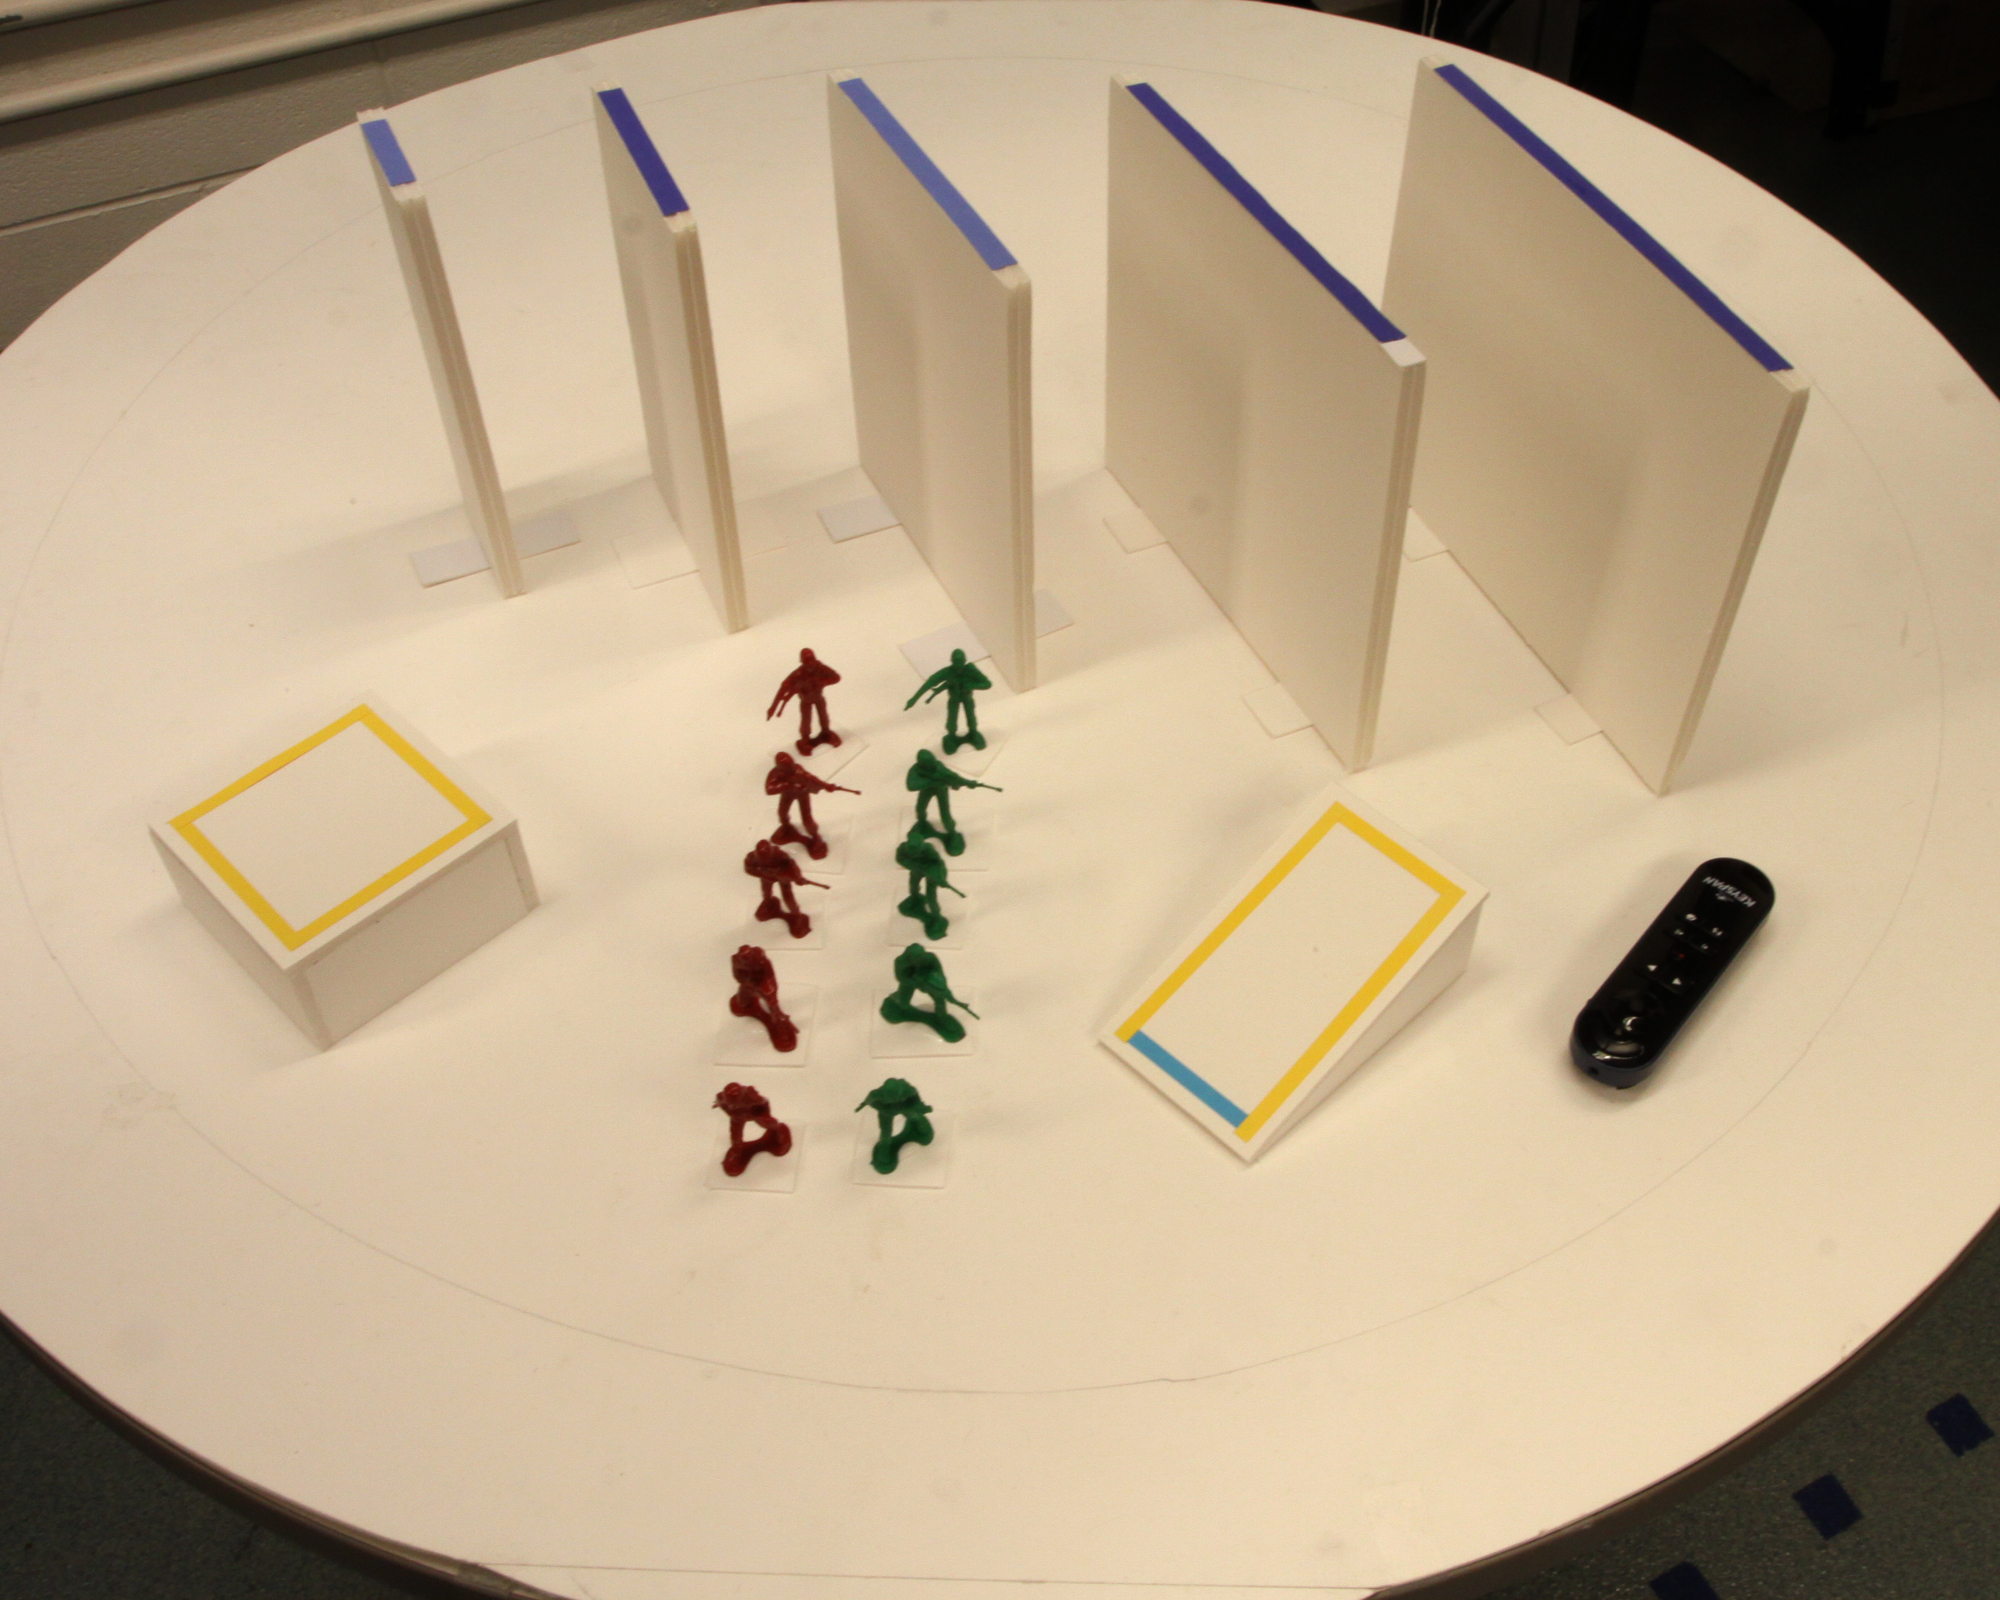
\includegraphics[width=4in]{images/props.jpg}
\end{center}
%\newcommand{\picwidth}{1.9in}
%\resizebox{\picwidth}{!}{\includegraphics{images/combat_movement_a.jpg}}
%\resizebox{\picwidth}{!}{\includegraphics{images/combat_movement_c.jpg}}
\vspace{-0.1in}
\caption[ARmy Primitives]{ARmy is played using a set of physical props and a simple wireless remote. The prop library contains plastic soldier figurines and foam-core terrain objects, including walls, platforms, and ramps}
\label{FIGURE:GamePrimitives}
\end{figure*}

In traditional miniature war games, players are typically allowed to represent terrain using whatever objects or methods may be available to them. However, many players prefer to use objects that physically resemble the terrain that they represent in order to make it easier for players to remember the meaning of each object. In addition, realistic terrain objects help to create a more aesthetically sound environment, which may help some players to feel immersed in the miniature world of the game. In this regard, techniques for spatial augmentation hold great promise as a means of flexibly applying a wide number of aesthetic choices to a single primitive object. The ARmy application uses the underlying SAR projection system to apply virtual textures directly onto the physical terrain primitives.  Figure~\ref{FIGURE:TerrainPlacement} shows a few example configurations under augmentation, with brick textures applied to the sides of elevated terrain, and a windowed building facade texture applied to the wall surfaces. Of course, these textures are merely an example of one possible aesthetic choice, and could easily be replaced with anything desired by the players, such as grass, concrete, or sandbags.

It is important to note that many players of miniature war games enjoy constructing and customizing terrain objects as much as they enjoy playing the game itself. For this reason, an ideal application of spatially augmented reality would not prohibit players from crafting and using such objects. In other words, visual augmentation is not intended to replace fine craftsmanship, but instead to be available only when players desire it. For example, consider a situation in which a player wishes to make last-minute changes to a setup, thus requiring him to add primitive objects to an otherwise highly-detailed scene. In this case, projecting a few well-chosen textures can help maintain the visual integrity of the game.

%FIGURE : TERRAIN DETECTION IMAGES
\begin{figure*}[t]
\begin{center}
\newcommand{\picwidth}{1.9in}
 \resizebox{\picwidth}{!}{\includegraphics{images/simple_lights_on.jpg}}
 \resizebox{\picwidth}{!}{\includegraphics{images/complex_no_walls_lights_on.jpg}}
 \resizebox{\picwidth}{!}{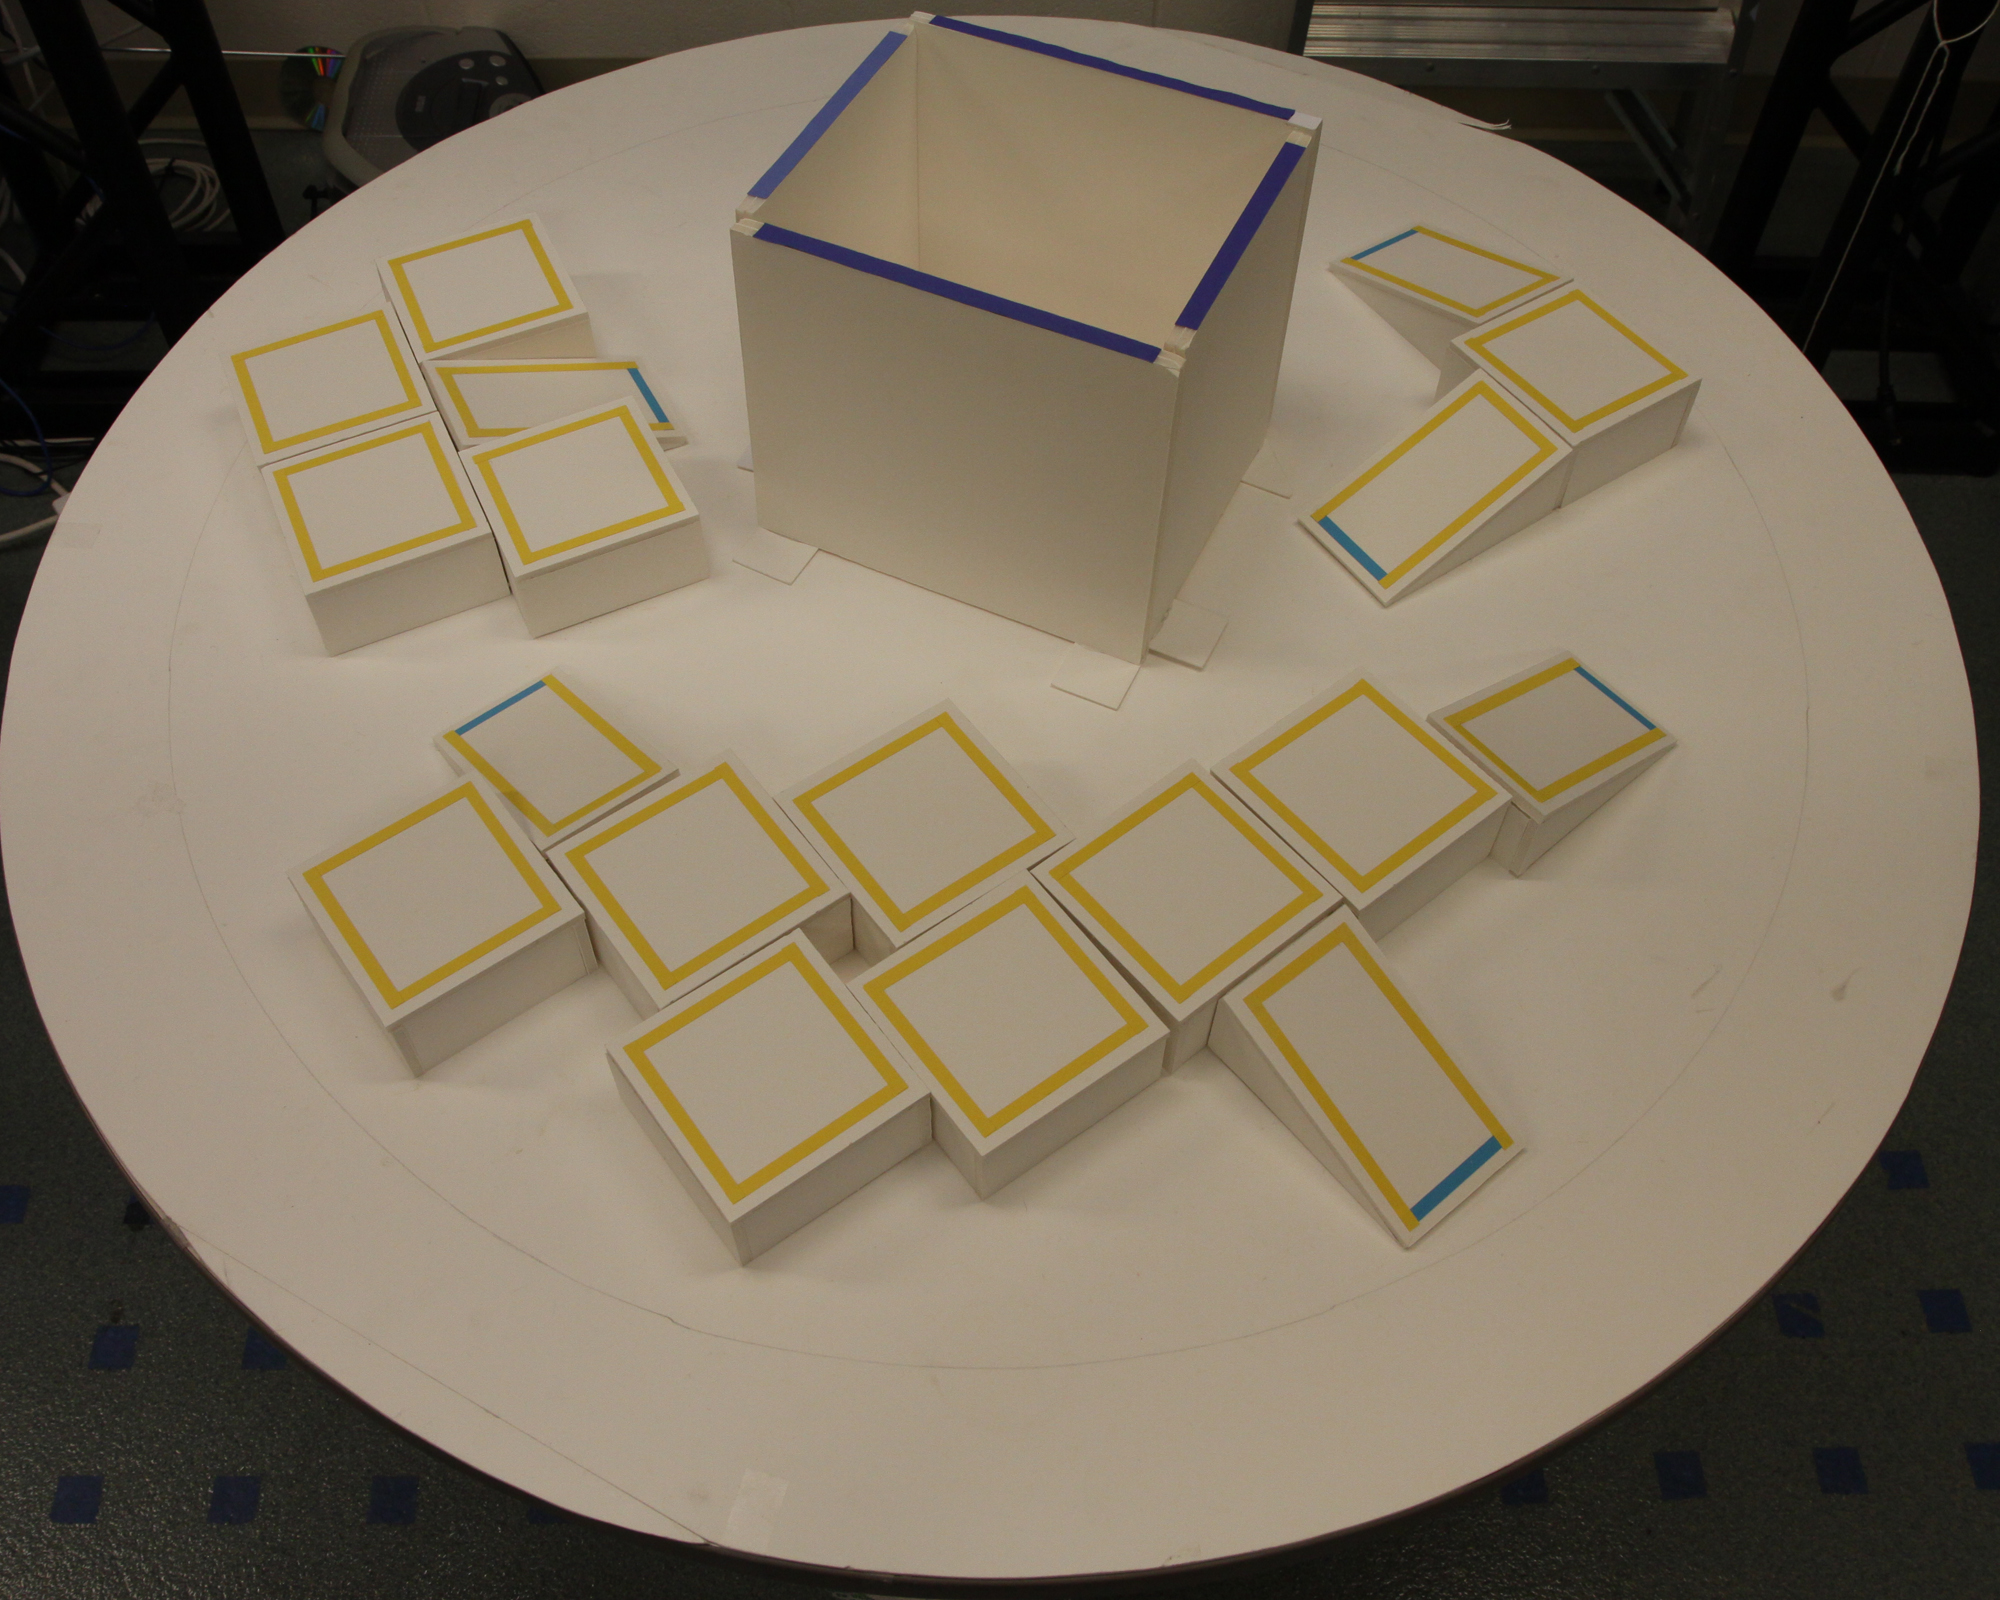
\includegraphics{images/complex_lights_on.jpg}}\\
\vspace{0.05in}
 \resizebox{\picwidth}{!}{\includegraphics{images/simple_projection.jpg}}
 \resizebox{\picwidth}{!}{\includegraphics{images/complex_no_walls_projection.jpg}}
 \resizebox{\picwidth}{!}{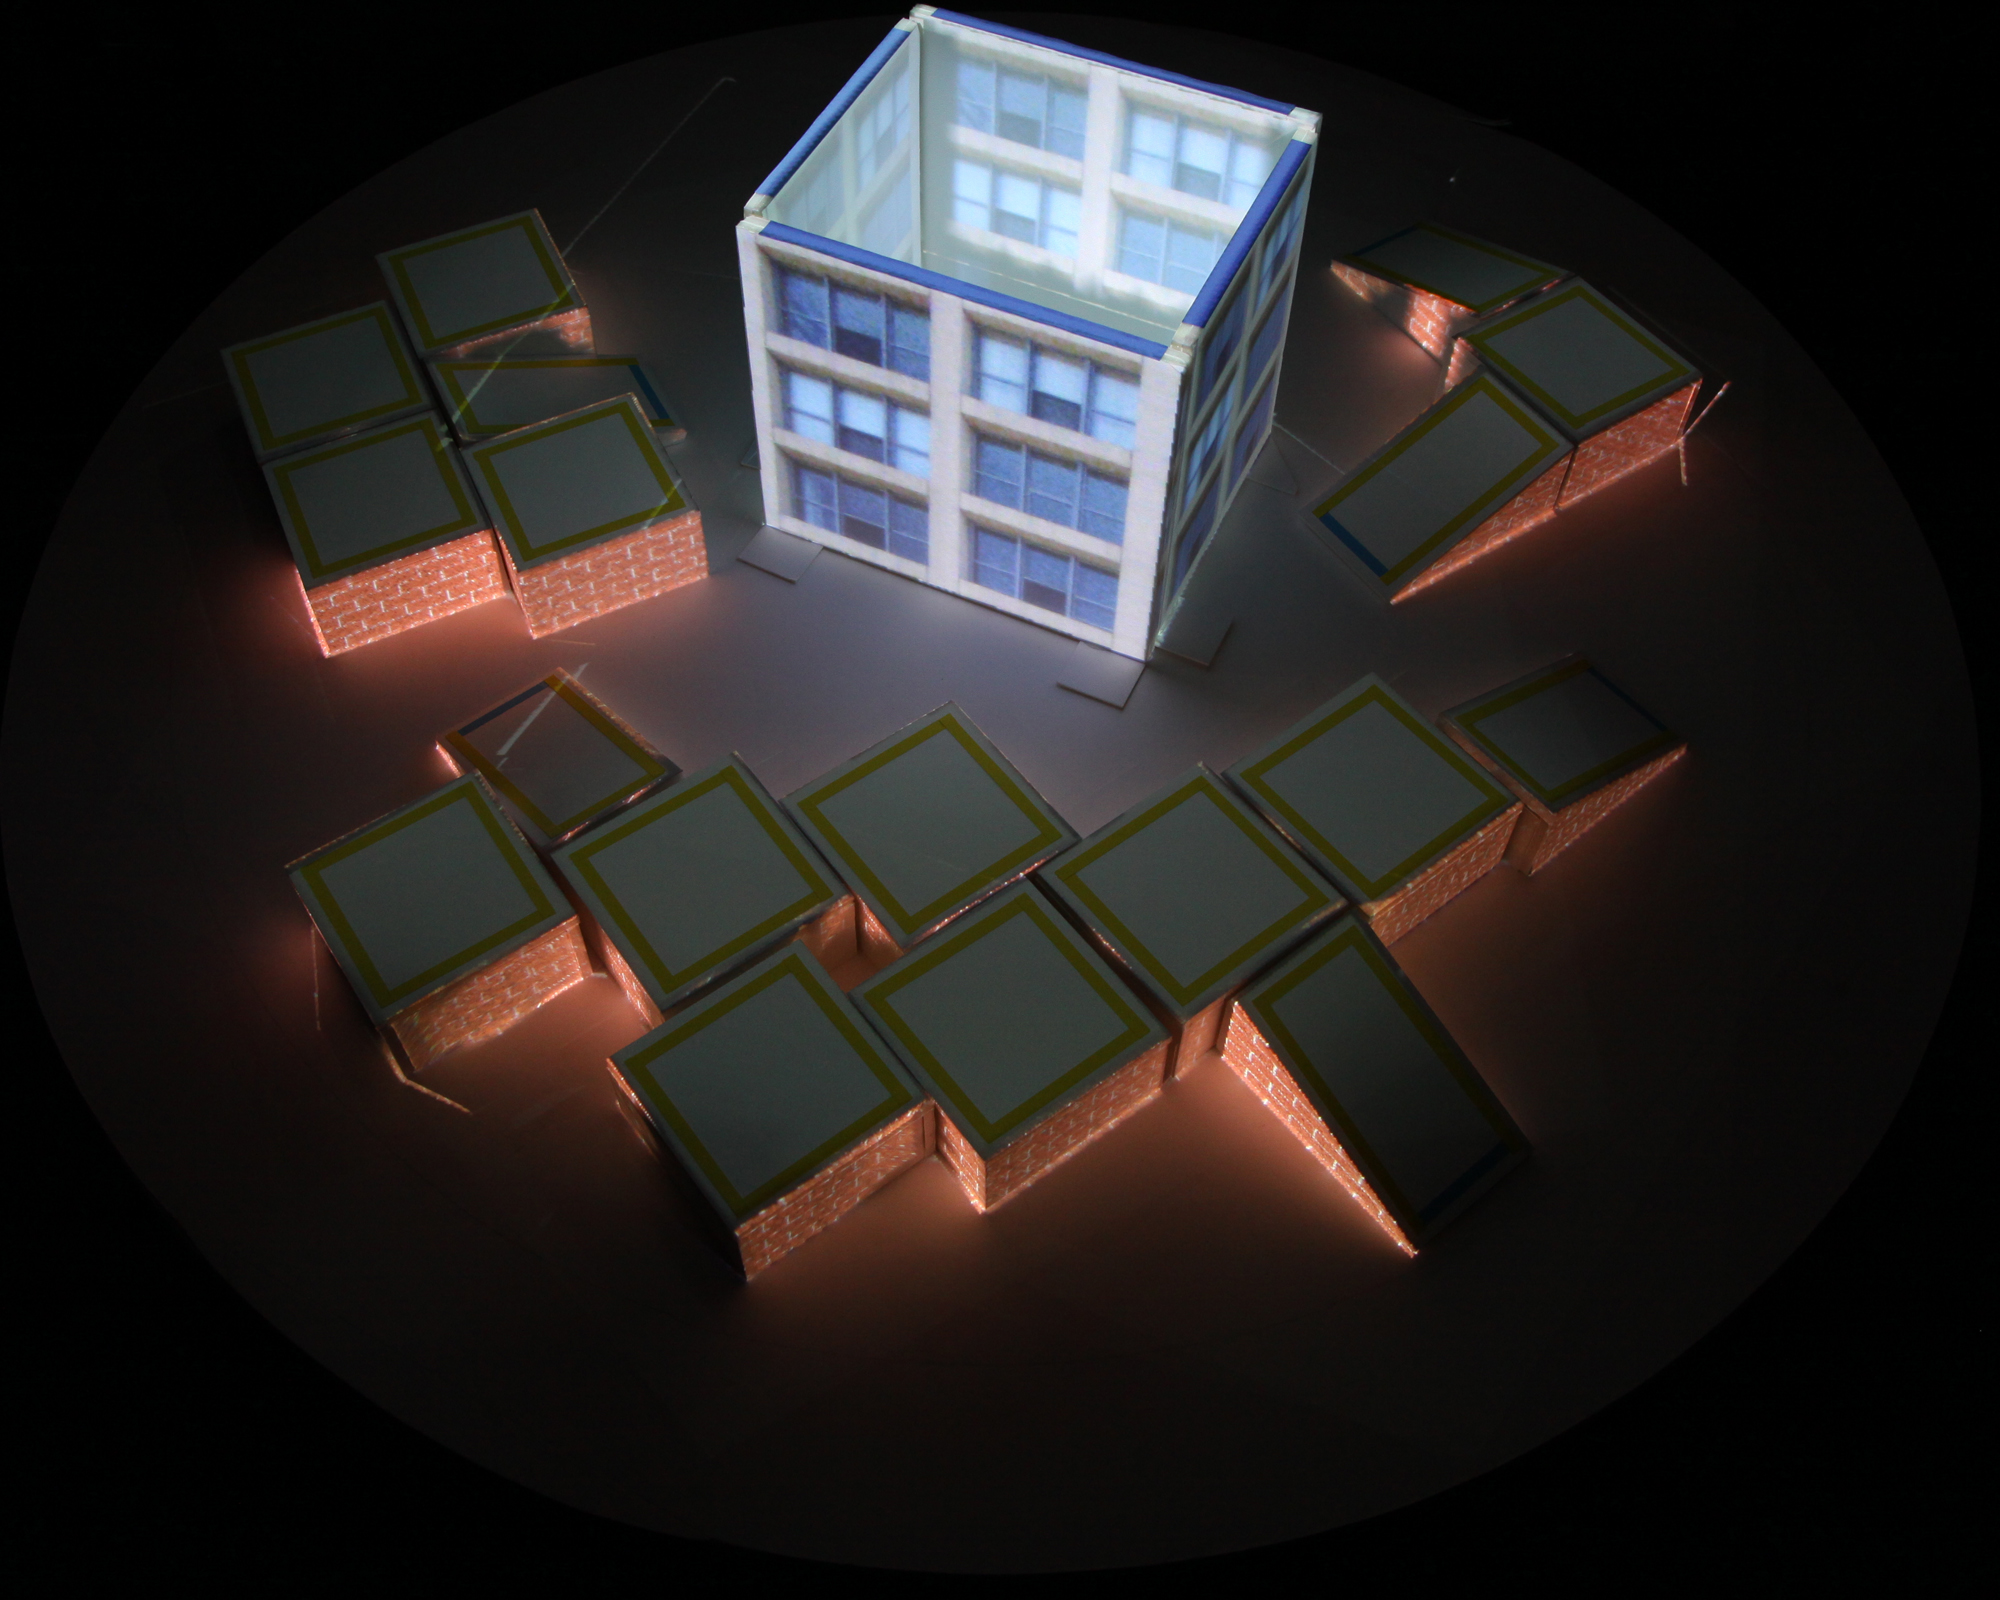
\includegraphics{images/complex_projection.jpg}}
\end{center}
\vspace{-0.1in}
\caption[Terrain Placement]{Players freely arrange terrain objects in the scene, and our system detects and augments these objects with virtual textures. Above are three example configurations, including a simple setup (left), a complex one (middle), and a more complex one with wall objects (right). }
\label{FIGURE:TerrainPlacement}
\end{figure*}

\subsection{Army Placement}

After configuring terrain, players decide on rules for positioning their respective armies. Units are represented using 2'' tall plastic soldier figurines, which have been colored with red or green spray paint to denote player ownership. As in any figurine-based tabletop game, units are positioned by physically placing them on the table. At any point during this step, players may request an update from the game module, which will then detect all positioned figurines, marking each with a colorful projected icon to show that it has been recognized, as depicted in Figure~\ref{FIGURE:CombatMovementExample}b. When all units have been placed and recognized satisfactorily, players signal for the game to start.

\subsection{Movement Phase}

Each player's turn consists of a \emph{movement phase,} during which he has the option of moving any number of his units. As in most tabletop war games, a unit's movement is constrained to a specified maximum distance, and must conform to the movement rules dictated by the terrain. However, a crucial difference is that in a traditional game, players would be required to measure distances using a ruler or measuring tape, and to make sure that all moves fall within the acceptable range. As previously stated, one goal of augmenting physical games with elements of video games is to automate tedious tasks that would otherwise burden the player, as well as subjective tasks that could lead to disagreements about legality. In this case, the game module completely eliminates the need for players to manually measure distances by precisely indicating each unit's field of movement, and reduces ambiguity in rules by notifying players when a move is illegal. Additionally, since players may move many units at once, the augmentation helps to indicate which units have already been moved from their initial positions, thereby avoiding a potential source of confusion.

% FIGURE OF EXAMPLE MOVEMENT REGIONS
\begin{figure}[t]
\newcommand{\picwidth}{2.9in}
\resizebox{\picwidth}{!}{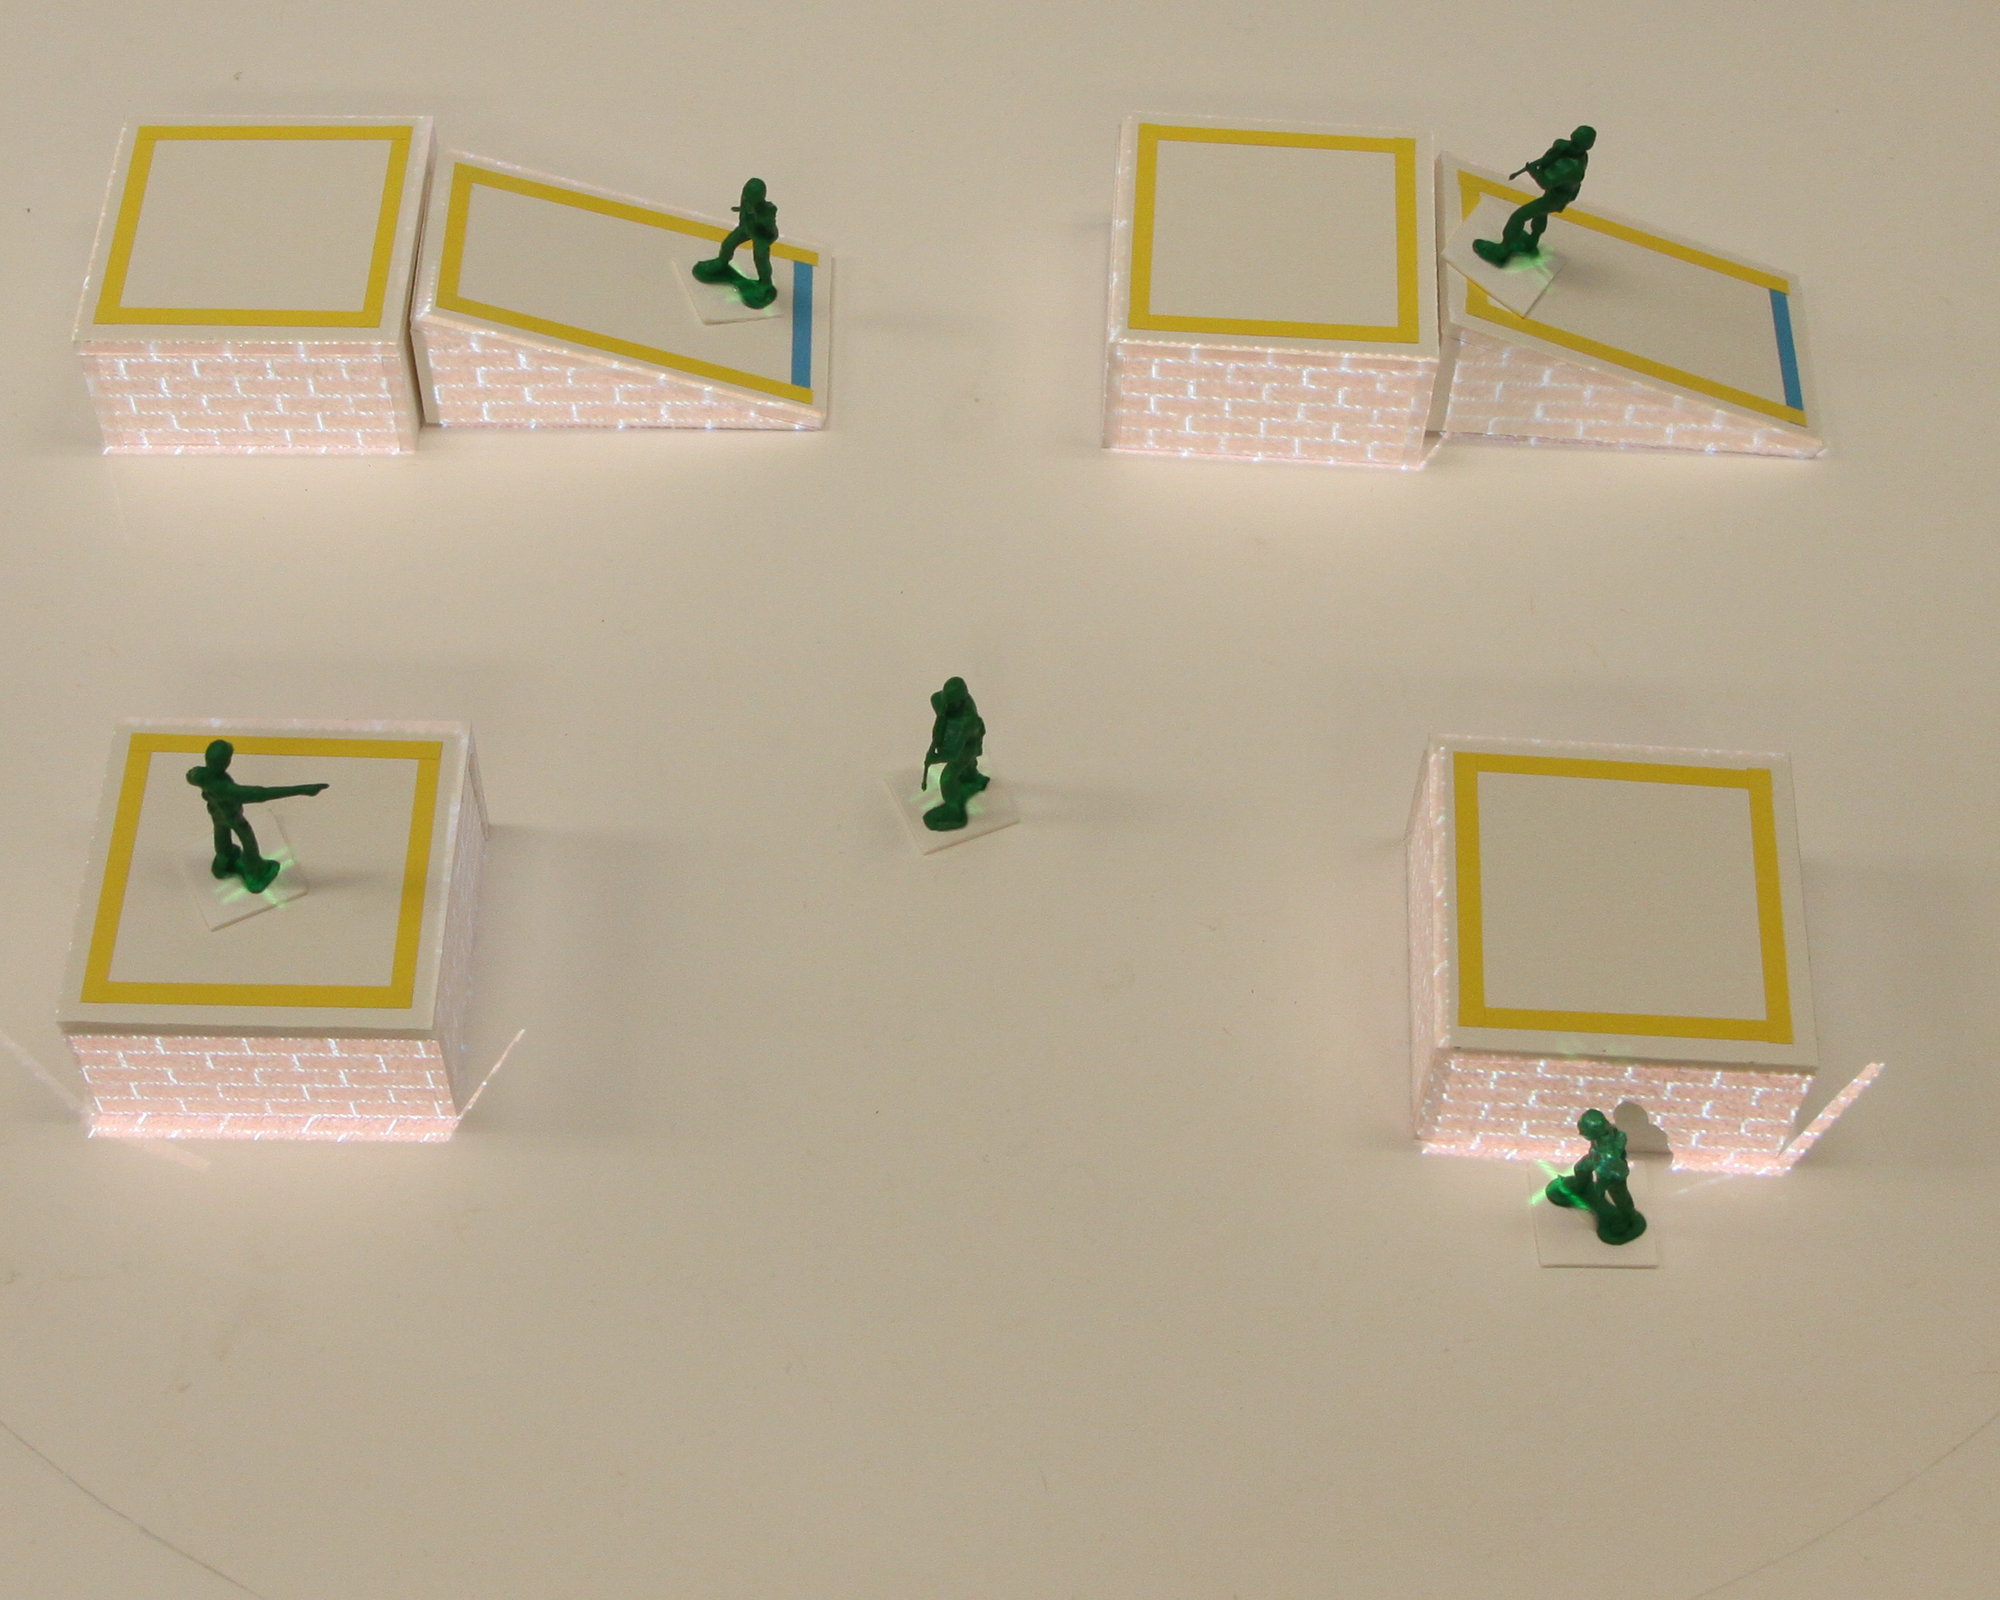
\includegraphics{images/movement_terrain_projection_lights_on_with_army.jpg}}
\resizebox{\picwidth}{!}{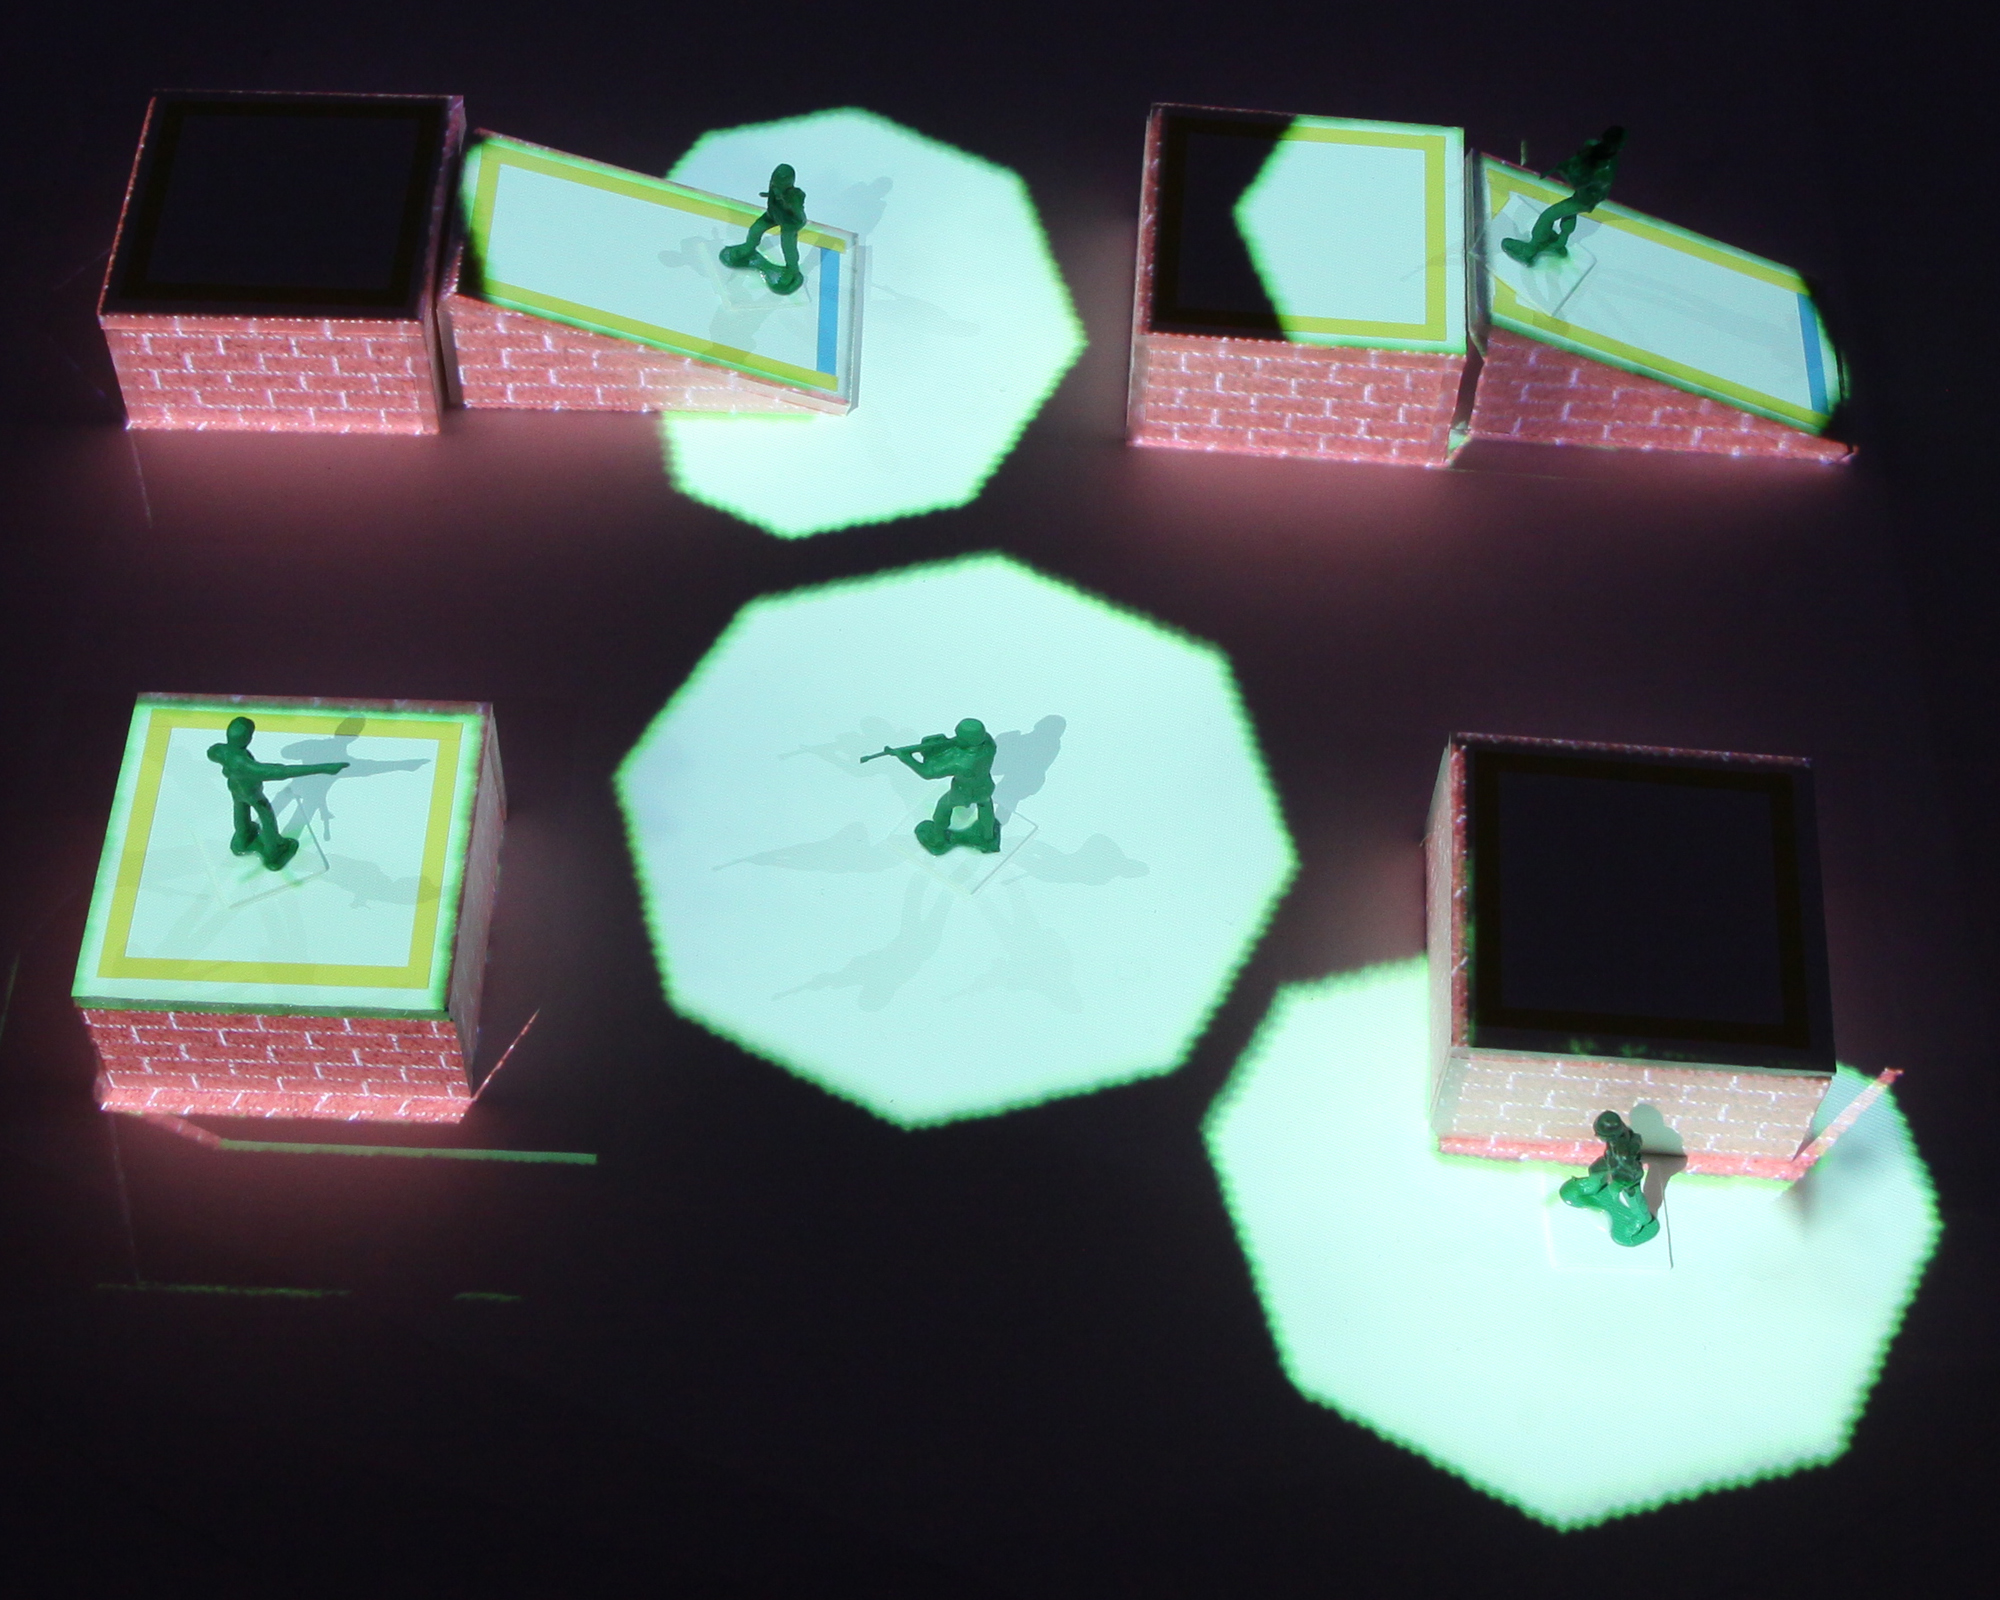
\includegraphics{images/movement_circles_projection.jpg}}
\caption[Movement Region Display]{\small{During a player's \emph{movement phase,} each unit's field of movement is illuminated. Note that each unit's movement field accounts for movement rules across terrain boundaries, which require the use of ramp objects in order to climb up or down elevated platform.}}
\label{FIGURE:MovementRegions}
\end{figure}

The exact steps of a movement phase are as follows. At the start of the phase, each unit's movement range is displayed as a colored region overlayed on top of the terrain (Figure~\ref{FIGURE:MovementRegions}). The player may move the unit anywhere within its corresponding highlighted region. At any point during the movement phase, the player may use the remote to request an update from the game module, which will then augment the overlayed display with a visualization of the desired moves. Each unit's current position is denoted by an ``\begin{math}\times\end{math}'' icon, while its original position at the start of the movement phase is denoted by an ``o'' %``\begin{math}\circ \end{math}'' 
icon. A bright connecting line is drawn between the two, marking the unit's movement path (Figure~\ref{FIGURE:CombatMovementExample}e). In the event that a given move is invalid, this information is reflected in the overlay by omitting the movement path line, allowing the player to correct the error (Figure~\ref{FIGURE:CombatMovementExample}d). The game continues to display the movement zones of each unit from its original position, in case the player changes his mind and would like to choose a different move for a particular unit (Figure~\ref{FIGURE:CombatMovementExample}g-h).

\subsection{Combat Simulation}
\label{SECTION:CombatSimulation}

\begin{figure*}[p]
\newcommand{\picwidth}{1.9in}
 \resizebox{\picwidth}{!}{\includegraphics{images/combat_movement_a.jpg}}
 \resizebox{\picwidth}{!}{\includegraphics{images/combat_movement_c.jpg}}
 \resizebox{\picwidth}{!}{\includegraphics{images/combat_movement_d.jpg}}
 %\resizebox{\picwidth}{!}{\includegraphics{images/combat_movement_d.jpg}}
 %\vspace{-0.20in}\\
 \begin{minipage}{\picwidth}\textcolor[rgb]{0,0,0}{\hspace{0.02in} {\bf a) initial setup}} \end{minipage}
 \begin{minipage}{\picwidth}\textcolor[rgb]{0,0,0}{\hspace{0.02in} {\bf b) with augmentation}} \end{minipage}
 \begin{minipage}{\picwidth}\textcolor[rgb]{0,0,0}{\hspace{0.02in} {\bf c) red's turn}} \end{minipage}
 %\begin{minipage}{\picwidth}\textcolor[rgb]{1,1,1}{\hspace{0.02in} %{\bf d) exact
%solution (+)}} \end{minipage}
 \vspace{0.04in}\\
 \resizebox{\picwidth}{!}{\includegraphics{images/combat_movement_f.jpg}}
 \resizebox{\picwidth}{!}{\includegraphics{images/combat_movement_h.jpg}}
 \resizebox{\picwidth}{!}{\includegraphics{images/combat_movement_n.jpg}}
 % QP simulated
 %\resizebox{\picwidth}{!}{\includegraphics{images/combat_movement_h.jpg}}
 %\vspace{-0.21in}\\
 \begin{minipage}{\picwidth}\textcolor[rgb]{0,0,0}{\hspace{0.02in} {\bf d) illegal move}} \end{minipage}
 \begin{minipage}{\picwidth}\textcolor[rgb]{0,0,0}{\hspace{0.02in} {\bf e) legal move}} \end{minipage}
 \begin{minipage}{\picwidth}\textcolor[rgb]{0,0,0}{\hspace{0.02in} {\bf f) green's turn}} \end{minipage}
 %\vspace{-0.13in}\\
 \vspace{0.04in}\\
 \resizebox{\picwidth}{!}{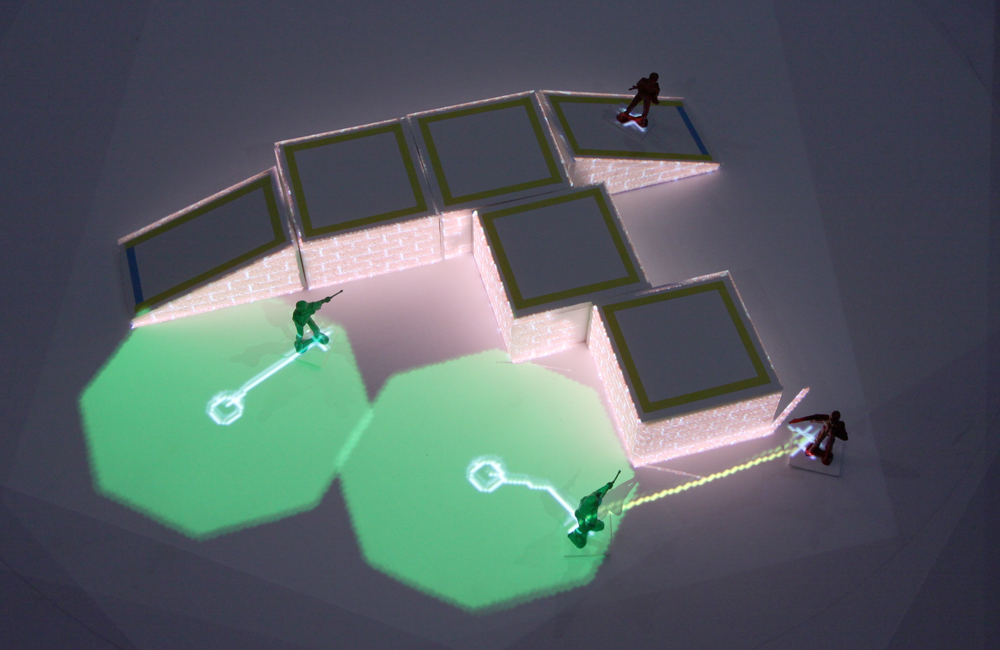
\includegraphics{images/combat_movement_p.jpg}}
 \resizebox{\picwidth}{!}{\includegraphics{images/combat_movement_r.jpg}}
 \resizebox{\picwidth}{!}{\includegraphics{images/combat_movement_t.jpg}}
 %\resizebox{\picwidth}{!}{\includegraphics{images/combat_movement_l.jpg}}
 %\vspace{-0.21in}\\
 \begin{minipage}{\picwidth}\textcolor[rgb]{0,0,0}{\hspace{0.02in} {\bf g) initial move}} \end{minipage}
 \begin{minipage}{\picwidth}\textcolor[rgb]{0,0,0}{\hspace{0.02in} {\bf h) revised move}} \end{minipage}
 \begin{minipage}{\picwidth}\textcolor[rgb]{0,0,0}{\hspace{0.02in} {\bf i) red's move}} \end{minipage}
 %\vspace{-0.13in}\\
 \vspace{0.04in}
 \resizebox{\picwidth}{!}{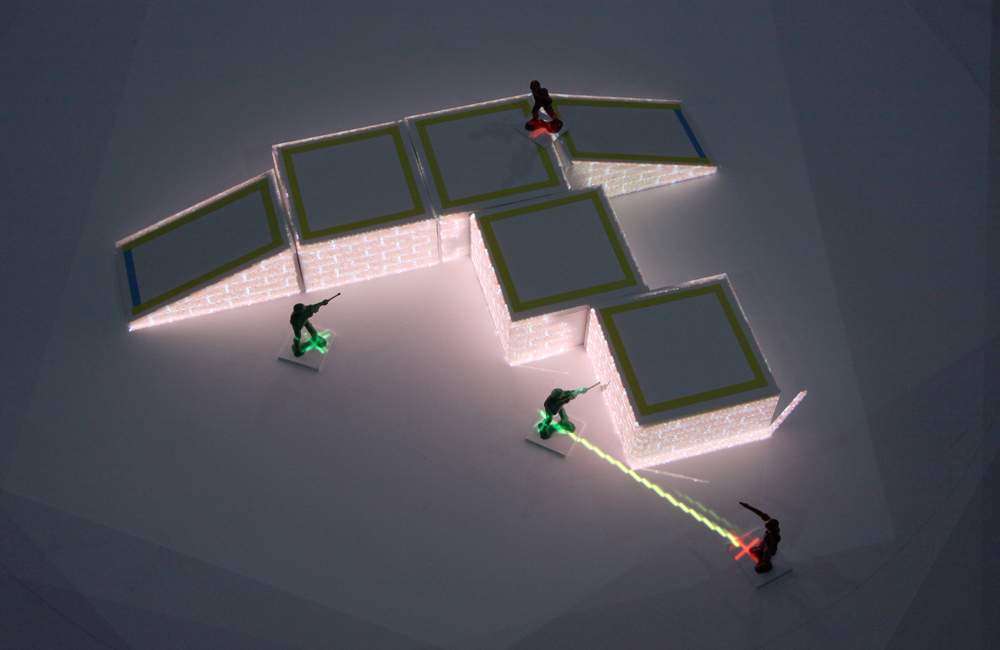
\includegraphics{images/combat_movement_u.jpg}}
 \resizebox{\picwidth}{!}{\includegraphics{images/combat_movement_v.jpg}}
 \resizebox{\picwidth}{!}{\includegraphics{images/combat_movement_w.jpg}}
 %\resizebox{\picwidth}{!}{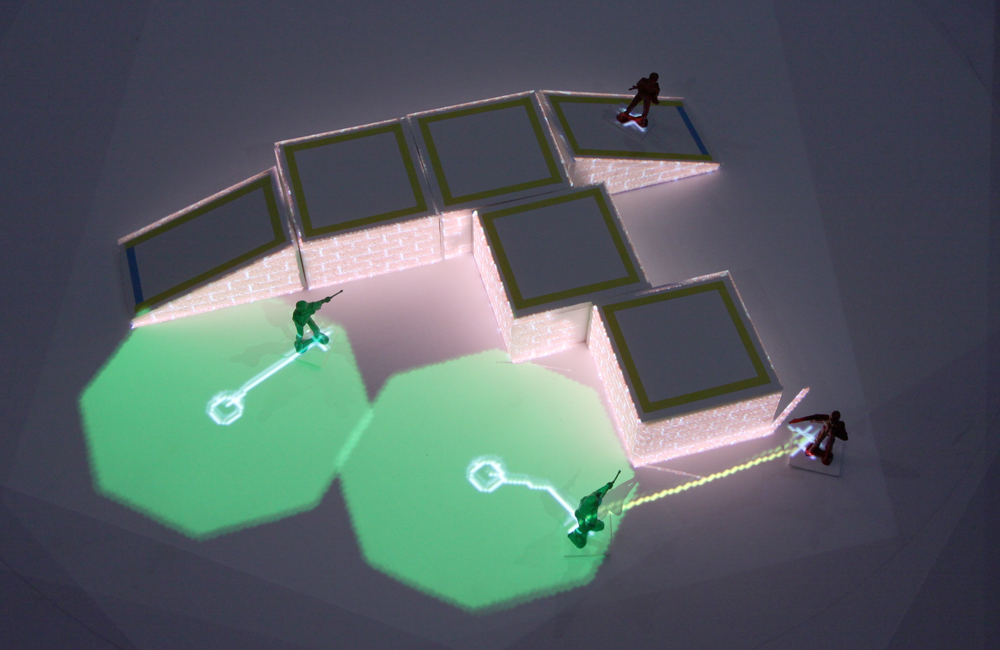
\includegraphics{images/combat_movement_p.jpg}}
 %\vspace{-0.21in}\\
 \begin{minipage}{\picwidth}\textcolor[rgb]{0,0,0}{\hspace{0.02in} {\bf j) combat}} \end{minipage}
 \begin{minipage}{\picwidth}\textcolor[rgb]{0,0,0}{\hspace{0.02in} {\bf k) red unit eliminated}} \end{minipage}
 \begin{minipage}{\picwidth}\textcolor[rgb]{0,0,0}{\hspace{0.02in} {\bf l) red unit removed}} \end{minipage}
\vspace{0.04in}
 \resizebox{\picwidth}{!}{\includegraphics{images/combat_movement_zd.jpg}}
 \resizebox{\picwidth}{!}{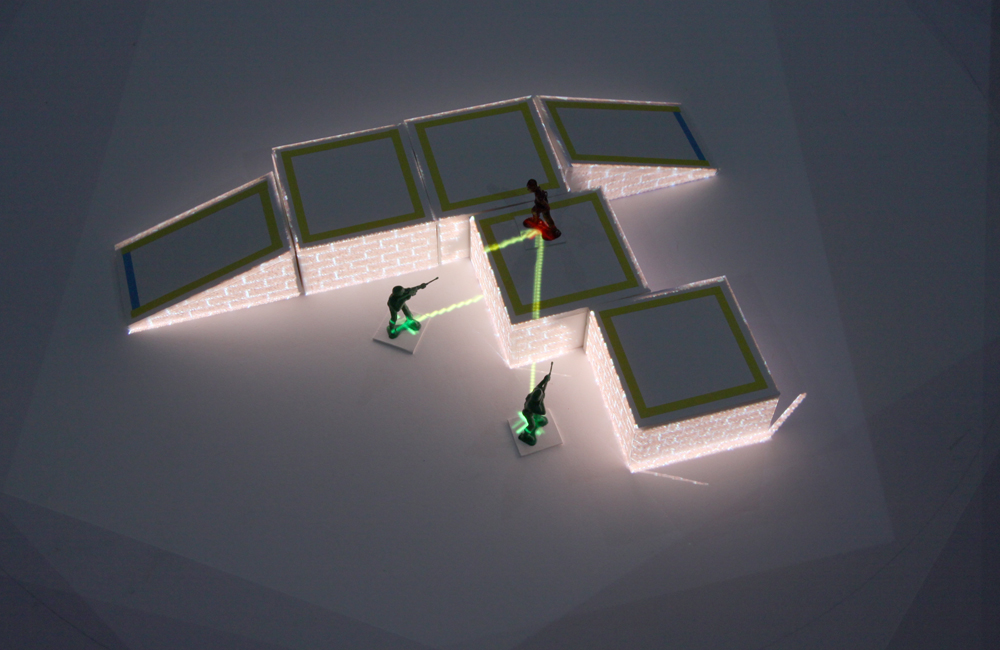
\includegraphics{images/combat_movement_ze.jpg}}
 \resizebox{\picwidth}{!}{\includegraphics{images/combat_movement_zg.jpg}}
 %\resizebox{\picwidth}{!}{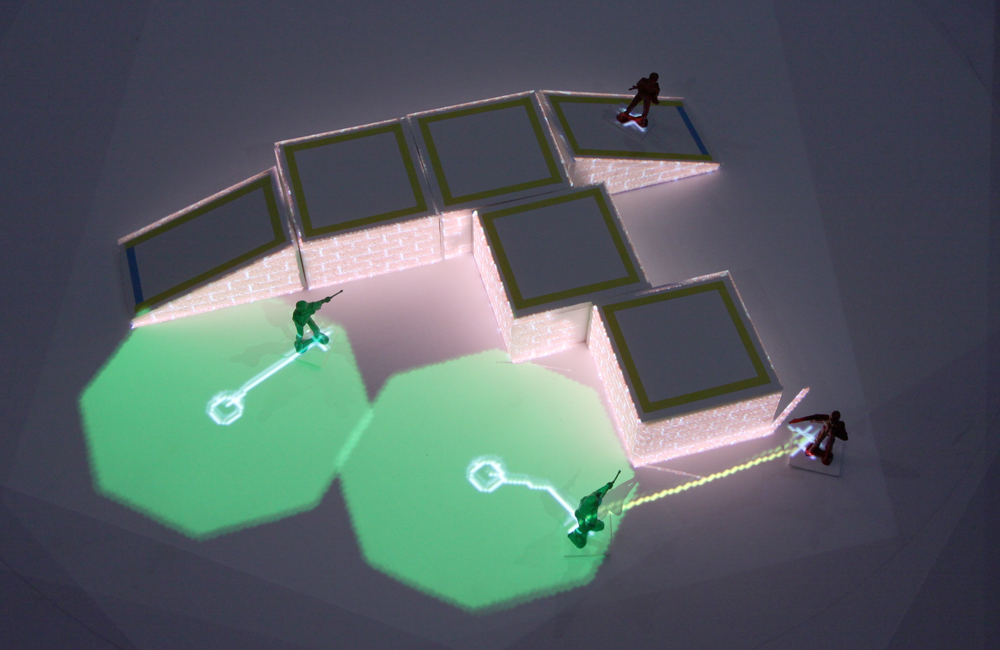
\includegraphics{images/combat_movement_p.jpg}}
 %\vspace{-0.21in}\\
 \begin{minipage}{\picwidth}\textcolor[rgb]{0,0,0}{\hspace{0.02in} {\bf m) green closes in}} \end{minipage}
 \begin{minipage}{\picwidth}\textcolor[rgb]{0,0,0}{\hspace{0.02in} {\bf n) final standoff}} \end{minipage}
 \begin{minipage}{\picwidth}\textcolor[rgb]{0,0,0}{\hspace{0.02in} {\bf o) green wins}} \end{minipage}

 %\vspace{-0.13in}\\
%
\caption[Sample ARmy Game]{Excerpts from a simple example game.}
\label{FIGURE:CombatMovementExample}
\vspace{-0.15in}
\end{figure*}



In addition to moving about the game world, tabletop war games require that units be able to engage other units in combat. Generally speaking, combat occurs when one player uses a particular unit to initiate an attack on an opposing unit. A unit that receives too many successful attacks is defeated and usually must be removed from play. Typically an attack can only be carried out across a specified distance range, and sometimes also requires that the attacker be able to ``see'' the target. In order to check that a valid line of sight exists between the two units, players often must crouch or lean over the table, align their eyes with the attacking figurine's ``point of view,'' and verify that the target figurine is visible and unobstructed by terrain or other objects. After a valid attack has been declared, its effectiveness is determined according to combat rules, which often involve rolling dice. Once again, all of these tasks represent prime opportunities for automation.

The current game prototype handles combat in a different manner from typical miniature war games, in that attacks are not explicitly declared by the players. Instead, each movement phase is followed by a \emph{combat simulation round,} during which all units automatically attack available targets in range. This is somewhat more similar to how combat works in a typical real-time strategy (RTS) video game, in which individual units exhibit a certain amount of autonomy in their actions, following orders only to the extent allowable by their preprogrammed behaviors. The idea of commanding ``smart'' units in combat interactions is not something that can be practically simulated by traditional tabletop war games, but is an interesting possibility for augmented reality games like ARmy. 

As players move units around the battlefield, yellow ``combat lines'' are overlayed on the ground textures, connecting opposing units that are able to attack each other (Figure~\ref{FIGURE:CombatMovementExample}j). This visualization provides important feedback to help players plan moves strategically. During a subsequent combat round, the game module iterates through all such connected pairs and in each case simulates an individual contest, which results in either one unit winning by successfully eliminating the other, or in a tie, in which case neither is eliminated. The contest consists of a simple ``dice roll'' calculation, which assigns each unit a probability value representing the likeliness of winning, weighted according to strategic advantages, such as holding higher ground than the opponent. At the end of the combat simulation round, units that have been eliminated are marked with a white ``\begin{math} \otimes\end{math}'' icon, signaling to the players that these figurines should be removed from play (Figure~\ref{FIGURE:CombatMovementExample}k). Once all eliminated units have been correctly removed, the players signal for the game to continue into the next movement phase.

\section{Large-scale Applications }

In addition to the small-scale tabletop AR system, our research group has developed a large-scale equivalent that aims to provide users with an immersive display environment~\cite{Yapo2010}. The differences between the two systems will be discussed later in the implementation details, but it should be mentioned that a key aspect of the large-scale system is its ability to continuously acquire updated views of the scene geometry while simultaneously displaying the AR visualization. In other words, while applications developed on the tabletop are typically updated only by user-driven commands, such as in the turn-based game detailed above, our large-scale applications are able to run continuously, responding to user actions at interactive rates. The applications discussed in this section were developed to explore and demonstrate the kinds of novel, tangible interactions that would be possible if everyday objects were augmented through similar SAR techniques.

\subsection { Ping Pong }

A prominent feature of our large-scale display environment is the use of full-size projection surfaces, which users may freely move in order to interact with the application and control the space. Many of the applications supported by our system utilize these surfaces as a means of user input to the system. For example, the original target application for our system is a lighting simulation for architectural design, which allows users to experiment with interior designs by using the projection surfaces as direct analogues to the physical walls of a room~\cite{Sheng2009}.

In line with this idea, we wanted to explore the possibility of using these surfaces as unorthodox game controllers. In developing such applications, we felt it absolutely critical that the function of the surfaces seem natural within the application setting, such that users may interact with the game intuitively and without detailed instruction. With this goal in mind, we developed a virtual ping pong game as a prototype application (Figure~\ref{FIGURE:pong}). The design was inspired by the iconic video game \emph{Pong}~\cite{Pong}, and strives to reimagine its classic interactions in the context of augmented reality.

\begin{figure}[t]
\includegraphics[width=\columnwidth]{images/pong.jpg}
\caption[Spatially Augmented Ping Pong Game]{ A game of immersive augmented reality ping pong.}
\label{FIGURE:pong}
\vspace*{-0.15in}
\end{figure}

As in traditional, real-life ping pong, the game is played between two opposing sides, each of which strives to bounce the ball past the opponent's paddle in order to score points. In this case, instead of using a table, the court is a large area of the floor, marked with a white rectangular boundary and a single dividing line drawn down the center. Like the court lines, the ball is a virtual element projected onto the floor. Each side is given a single movable projection surface, which acts as a paddle. When the ball intersects the bottom of a paddle surface, it is deflected off in a direction consistent with the surface angle. Because it is easier for a pair of users to manipulate a surface when working together than it is for a single user, the game is typically played with teams of two. Each paddle surface is augmented to display its corresponding team's color, and additional projection surfaces located outside of the play area are used to display each side's current score.

\subsection { Laser Pen Applications }

Although a wide variety of applications are possible using the physical interactions of the projection surfaces alone, we felt that in many cases users would benefit from the ability to interact with virtual elements in the scene using a more precise means. Recent work on our system has introduced the use of laser pens to allow users to point directly at displayed objects for a variety of interactions. The devices used are commonplace green laser pens, typically used for pointing during presentations. Overall, we find that the laser pen interface provides an excellent way for users to perform tasks both independently and cooperatively across the wide display area of our large-scale system.

In particular, I developed a simple shooting gallery game in which players use laser pens to hit targets projected on the walls and floor. Figure~\ref{FIGURE:SpaceInvaders} shows the game using only the floor and back wall surfaces, but the application could be easily extended to incorporate additional surfaces. Targets are generated at random locations along the top portion of the wall and move downwards at varying angles. Upon reaching the bottom of the wall, each target moves across the floor until it passes the end of the playing field, at which point it is considered a missed target. As play continues, the game increases the rate of target generation and introduces faster targets with more complex zig-zag patterns in order to increase difficulty. The mechanics and overall feel of the game are inspired by the style of ``retro'' video games, most notably the arcade classic \emph{Space Invaders}~\cite{SpaceInvaders}. Overall, the game is fun and intuitive, and acts as an interesting ``warm-up'' for new users by allowing them to practice with the laser pen interface before moving to applications with potentially more complex interactions.

\begin{figure*}[t]
\newcommand{\picheight}{2.05in}
 \resizebox{!}{\picheight}{\includegraphics{images/space_invaders_3.jpg}}
 \resizebox{!}{\picheight}{\includegraphics{images/space_invaders_2.jpg}}
\caption[Spatially Augmented Shooting Gallery Game]{A large-scale shooting gallery game in which the user aims at virtual targets with a laser pen.}
\label{FIGURE:SpaceInvaders}
\end{figure*}

\section{Summary}

In summary, my work has focused on the development of a number of applications supported by both our small-scale and large-scale spatially augmented reality display systems. The ARmy application builds upon the basic concept of a physical tabletop war game by introducing virtual game elements. The advantages of this method are that it provides an intuitive interface and display, allowing players to easily see available options, and that it automates a number of tedious tasks that might ordinarily encumber play, such as measuring distances, checking lines of sight, and performing arithmetic for calculations in combat. The large-scale applications explore possible ways in which users may interact with our system, by directly moving physical projection surfaces to alter the scene, and by using laser pointers to precisely interact with virtual elements.

\chapter{IMPLEMENTATION DETAILS }

\footnote{Portions of this chapter previously appeared as: Theodore C. Yapo, Yu Sheng, Joshua Nasman, Andrew Dolce, Eric Li, and Barbara Cutler. Dynamic Projection Surfaces for Immersive Visualization. PROCAMS 2010 IEEE International Workshop on Projector-Camera Systems, June 2010.}

The spatially augmented reality game applications presented in the previous chapter are built on top of a system for dynamic projection developed through ongoing work by members of our computer graphics research group. The purpose of this chapter is not to explain the details of our system in depth, but rather to provide a general overview of how the system is organized, and to explain how each of the existing components is used to create the game applications. I will highlight the algorithms that I personally contributed to the system infrastructure and I will also explain how I prototyped the game applications by adapting and extending portions of the system developed by other students.

\begin{figure*}[t]
    \includegraphics[width=\textwidth]{images/system_diagram.pdf}%
%\vspace{-0.25in}\\
    \caption[Overview of System Architecture]{
%
The architecture of our system is composed of several asynchronous
computation modules. The \emph{vision} component detects objects in the camera images and produces skeleton geometry, which is converted to a continuous mesh by the \emph{world modeling} component. A distributed rendering process driven by the \emph{display controller} sends the data across a local gigabit Ethernet network to multiple projection servers, each of which handles up to four \emph{projector renderers.}}
\vspace{-0.15in}
\label{FIGURE:block_diagram}
\end{figure*}

\section{System Overview}

Although our small-scale and large-scale systems differ in a number of ways, the two can be understood as variations of a single design, divided into a number of components. The purpose of this section is to provide a high-level outline of this system, describing the role of each individual component.

An important principle of the general system design is that each component represents a single autonomous process. Since the various responsibilities of a given component may require it to run at different rates than others, we decouple them such that at any point in time, a process can obtain the latest output from the previous stage of the pipeline (Figure~\ref{FIGURE:block_diagram}). 

\subsection{Camera Component for Scene Recognition and Tracking}

Projecting images onto a dynamic scene requires that our system be able to accurately recover the positions and orientations of objects and surfaces as they move. We achieve this by tracking objects using images captured from a single camera mounted in an overhead position. The camera hardware is capable of capturing and transmitting 1280\begin{math}\times\end{math}960 pixel images through a gigabit Ethernet connection at 33 frames per second. Since the camera remains stationary during system use, we recover both intrinsic and extrinsic calibration parameters as a precomputational step. The small-scale system uses Zhang's method of calibration~\cite{Zhang2000}, while the large-scale system uses Scaramuzza's calibration model~\cite{Scaramuzza2006} for correcting distortion, since we equip the camera with a fisheye lens in order to increase the area of coverage.

\subsection{Vision Component }

The \emph{vision component} is responsible for processing the raw camera output in order to achieve 3D registration of objects in the scene. Of all the system components, the vision module is the one that differs most between the two system variants. Because each system is built with different goals and constraints, each uses a completely different method for detecting objects. In the large-scale system, we identify projection surfaces by tracking a number of embedded infrared LED markers, allowing us to ignore information in the visible light spectrum. This is important because our large-scale system is built with the goal of achieving simultaneous acquisition and display to facilitate real-time applications. In contrast, the small-scale system does not provide this feature, and instead detects objects using simple colored markers, making the objects lighter, cheaper, and easier to construct. In either case, the output of the vision module is a list of detected objects and associated positional data, which we refer to as the ``skeleton geometry'' of the scene.

\subsection{World Modeling Component }

Skeleton geometry alone generally does not provide a sufficient representation of the scene for augmentation. Instead, this information is passed to the \emph{world modeling component}, which is responsible for constructing a more complete environment model in order to suit the needs of the rendering modules, and sometimes the application. The output is a three-dimensional virtual model of the scene in the form of a triangle mesh. Additionally, two-dimensional heightfield representations of the scene can be provided if needed by a particular application. 
%Additionally, this module uses projector calibration data to compute %a set of blending weights used to smooth variations in intensity %across regions of projector overlap.

\subsection{Display Controller and Projector Renderers }

Because the number of projectors that a particular machine may drive is limited to the number DVI output ports that it provides, our system uses a distributive rendering process to divide the workload across multiple computers. Our most recent configuration is capable of driving a maximum of eight projectors by using two servers, each equipped with two dual-head graphics cards. We accomplish this using a single \emph{display controller,} which coordinates a number of remote \emph{projector renderer} modules. The display controller sends relevant display information to the separate renderers, including the geometric model and textures. Each projector renderer controls the display of a single projector and generates the final display image by rendering the virtual model of the scene from the perspective of the projector based on calibration data.

\section{ARmy Application Details }

The ARmy application was built on top of the small-scale version of our system. This section explains in greater detail the ways in which the application interacts with the underlying system modules, as well as the algorithms used to perform various game operations.

\subsection{Object Detection }

%FIGURE : Object detection images

\begin{figure*}[p]
\begin{center}
\newcommand{\picwidth}{2.3in}
 \resizebox{!}{\picwidth}{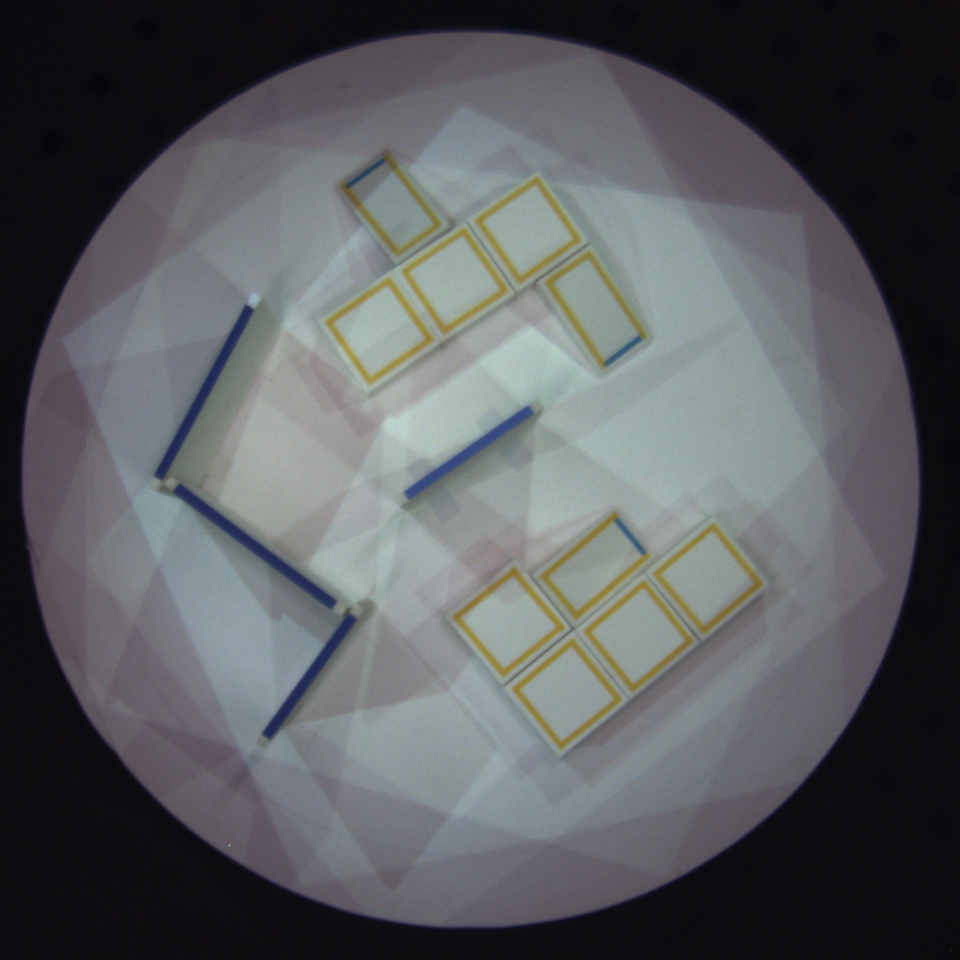
\includegraphics{images/detection_images/raw.png}}
 \resizebox{!}{\picwidth}{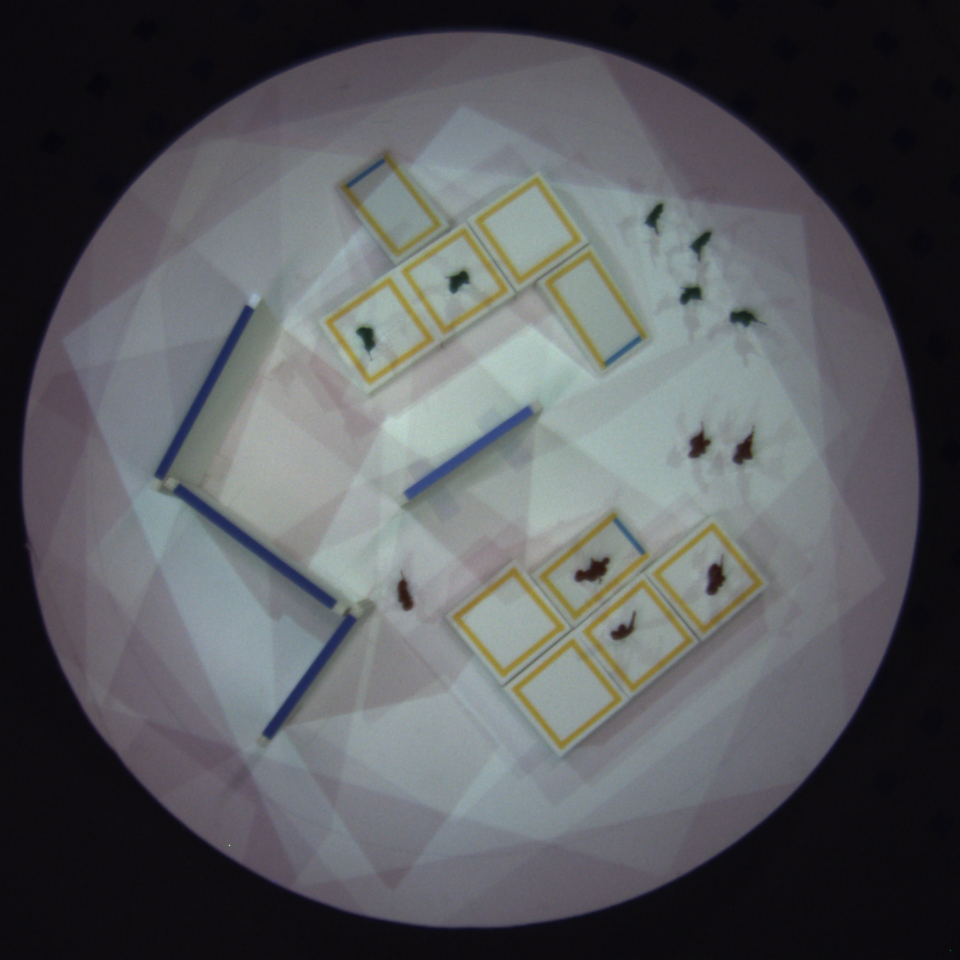
\includegraphics{images/detection_images/raw_with_soldiers.png}}\\
 \resizebox{!}{\picwidth}{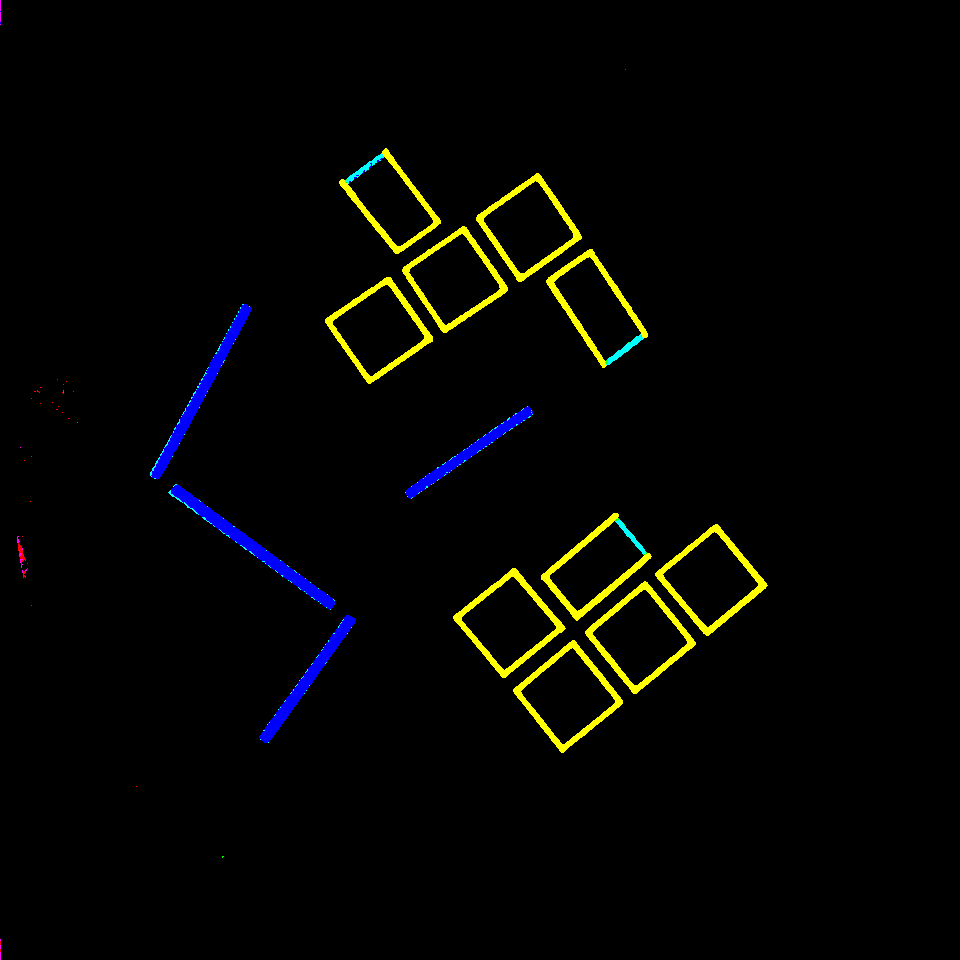
\includegraphics{images/detection_images/enh_colors.png}}
 \resizebox{!}{\picwidth}{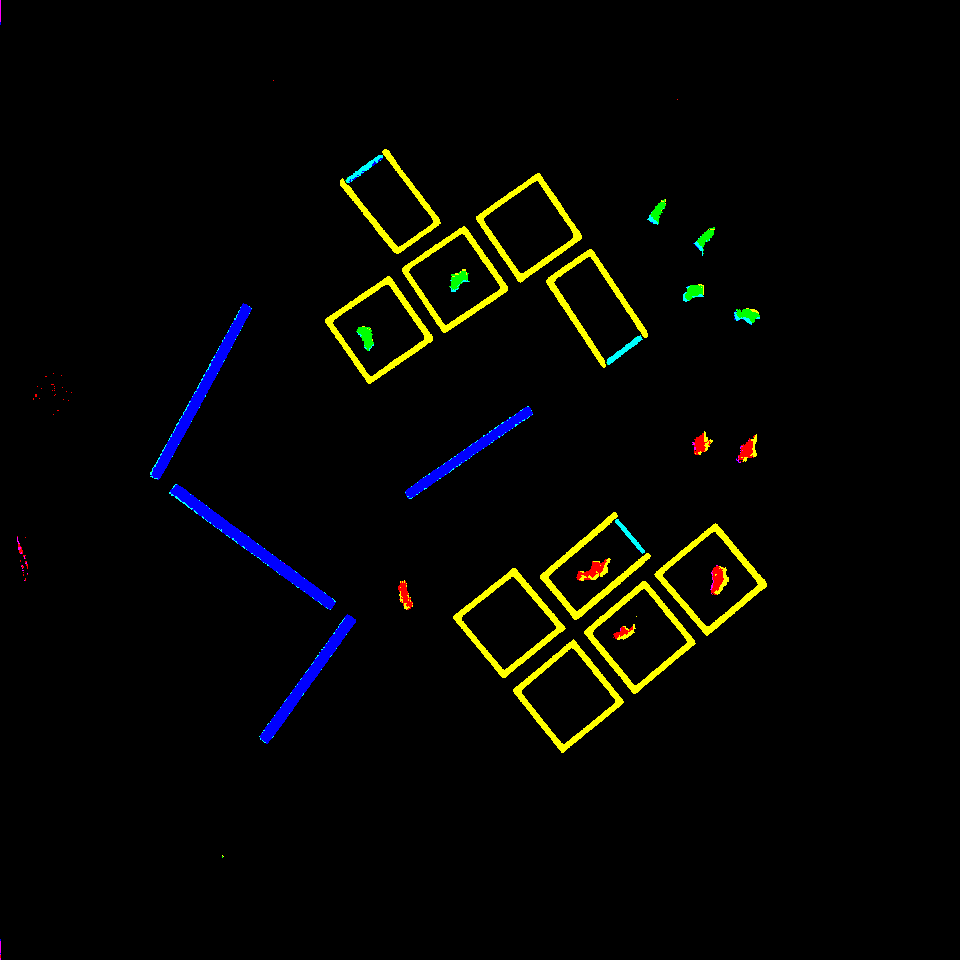
\includegraphics{images/detection_images/enh_colors_with_soldiers.png}}\\
 \resizebox{!}{\picwidth}{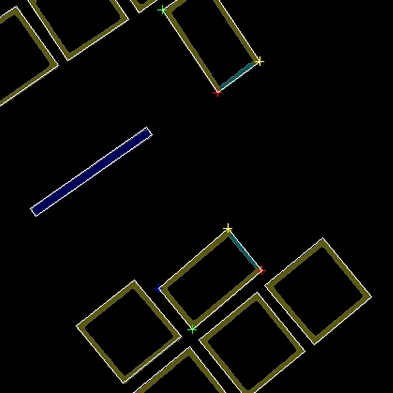
\includegraphics{images/detection_images/terrain_labels_crop.png}}
%\resizebox{!}{\picwidth}{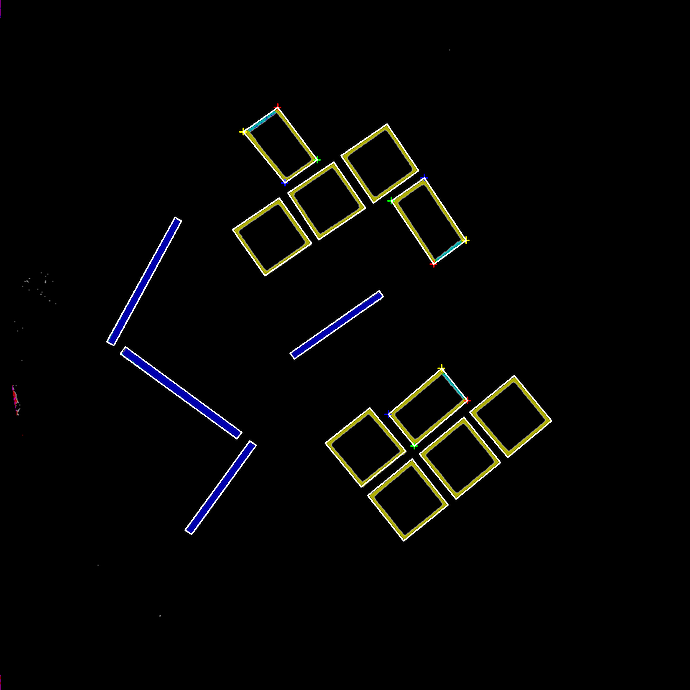
\includegraphics{images/detection_images/terrain_labels_bright.png}}
 \resizebox{!}{\picwidth}{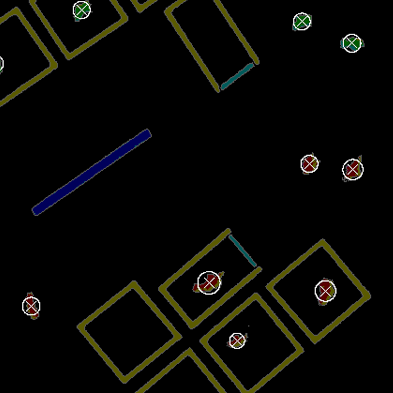
\includegraphics{images/detection_images/labels_with_soldiers_crop.png}}
\end{center}
\vspace{-0.15in}
\caption[ARmy Object Detection]{Raw camera images of the scene (top) show variable lighting due to shadows and regions of projector overlap. The \emph{vision component} ignores these artifacts by considering only pixels with highly saturated color properties, which it groups into connected components (middle.) These components are classified as quadrilateral terrain regions (bottom left) or soldier figurines (bottom right) based on size, color, and shape.}
\label{FIGURE:ARmyObjectDetection}
\end{figure*}

%Our SAR tabletop system detects objects using a single calibrated %camera mounted overhead for a top-down viewpoint. 
During acquisition, a single image from the camera is processed by our vision module, which uses thresholding techniques to identify connected image components with predominant color attributes matching a set of identifiable colors. Currently the set is limited to six colors : red, green, blue, yellow, cyan, and magenta. This six-color vocabulary has proven sufficient for a number of applications developed using the system.

After a colored component is detected, the vision module attempts to classify it as a known object type based on a set of rules dictated by the current application. In the case of the ARmy application, the vision module is equipped with a set of rules specifically tuned for detecting the game object primitives. Because the game is designed with the assumption that terrain does not change beyond the initial setup phase, which occurs before soldier units have been placed in the scene, the classification rules can be separated into two distinct sets, allowing the vision module to operate in separate modes. 

The first mode is used only in the terrain placement phase of the game to detect the initial configuration of terrain objects, which are encoded with the colors blue, yellow, and cyan. Blue components that fit a rectangular shape within an acceptable margin of error are classified as wall objects. Platform objects are detected in the image as yellow components with a valid quadrilateral fit. Similarly, ramps are classified from quadrilateral components with three predominantly yellow sides and one predominantly cyan side. The cyan side indicates the low edge of the ramp, which reaches down to the table surface. Once an appropriate quadrilateral has been fit to a terrain object, the corners are used to specify position and orientation.

After the terrain setup has been finalized, subsequent scene recognition steps use the second detection mode, which is responsible for identifying soldiers. Since red and green colors are reserved for soldier figurines, any red or green component that falls within an acceptable range of sizes can be classified as a soldier unit. Each detected unit is assigned a single location equal to the centroid of the component in image space.

In either case, any detected component that does not fit a specified classification rule is deemed irrelevant and discarded. Once a component has been classified as a valid object, its known world dimensions are used in combination with the calibration data of the camera to determine its position and orientation in world space. For any given pixel coordinates in the camera image, the calibration parameters define a ray in 3D space representing the corresponding path along which light enters the camera. By using the known height of the object at that point, we can backproject along the ray to determine the exact world position.

Overall, our color-based detection method successfully recognizes a variety of objects without the need for large fiducial markers or embedded sensors, allowing us to easily construct a sizeable collection of lightweight objects. Objects with natural color properties, such as brightly colored game pieces, can often be tracked without any modification, while objects that lack these properties can be tracked with the simple addition of colored markers.

%\subsection{ Virtual Modelling of the Scene}

%As discussed in the system overview, our \emph{world modelling} %component is capable of constructing both 2D and 3D virtual %representations of the physical scene. The ARmy game application uses

%In order for our system to dynamically project on the detected %objects, it is necessary that we compute a virtual model of the %scene. This step is handled by a different system component, which %receives the positional data of the detected objects and outputs a %three-dimensional mesh that closely matches the real-world geometry. %In addition, this module is capable of outputting a two-dimensional %heightfield of the scene, a feature that is utilized by the ARmy game %in order to obtain a simplified representation of the game world.

%\fbox{Mention texture stuff here? Special-case UVs for floor?} \\
%\fbox{Also, does it sound like I'm taking credit for this?}

\subsection{Modeling the Game World }

The game world is represented as a two-dimensional heightfield, discretized into a high-resolution square grid. The purpose of this grid is to allow the game module to approximate the travel distances of units as they move through the scene, as well as to perform line-of-sight checks for combat purposes. In addition to a height value, each cell stores the cost of moving from the cell to each of its eight neighbors, subject to a maximum height difference threshold. If the difference in height of two adjacent cells is below the threshold, then the cells are considered connected neighbors, and the associated movement cost is equal to the Euclidean distance between the two, which is simply 1 for neighbors along cardinal directions and \begin{math}\sqrt2\end{math} for diagonal neighbors. If the height difference is above the threshold, then it is impossible for a unit to move between the two, and therefore the distances are set to infinity. 
Because the terrain configuration does not change after the terrain placement step, these distance values are computed once for all cells and stored for the remainder of the game. Since each cell is connected to at most eight neighbors, the average size of the data per cell is invariant with respect to the number of cells in the grid, which means that this method scales reasonably to higher resolutions.

The result of this process is a connected graph that reflects the kind of movements expected according to the rules of the game. Units may follow paths that traverse flat terrain regions, as well as ramps, which exhibit smooth height variations, but may not pass through sharp boundaries, such as cliffs and walls. More complex movement rules could be integrated simply by changing the rules for assigning movement distances between neighbors. For example, we could add a rule that soldiers move more slowly when walking up a ramp than when walking down one, by assigning costs asymmetrically between connected neighbors according to height differences. The only requirement is a means of initializing the heightfield to accurately represent the terrain configuration constructed by the players.

As mentioned in the system overview, the world modeling component of our system is capable of providing a suitable heightfield rendering of the scene. However, initializing the values of the grid from this raw heightfield output creates a few problems. In fact, this height information is too accurate, in that it often captures tiny discontinuities that players would generally want to ignore. For example, consider two platform objects that are placed side by side such that they are nearly touching, with the intention that units be able to move freely between the two. Unfortunately, a thin crevice still exists between the two that is likely to be reflected in the raw heightfield. If unaltered, this feature would result in an impassable barrier, defeating the intended purpose of the terrain configuration.

% FIGURE: HEIGHTFIELD OPERATIONS
\begin{figure*}[t]
\newcommand{\picwidth}{1.9in}
\begin{center}
 \resizebox{\picwidth}{!}{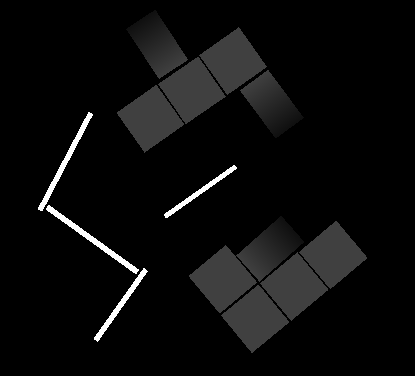
\includegraphics{images/heightmap_vis/initial_heightmap.png}}
 \resizebox{\picwidth}{!}{\includegraphics{images/heightmap_vis/floor_start.png}}
 \resizebox{\picwidth}{!}{\includegraphics{images/heightmap_vis/floor_dilated_diff.png}}  \vspace{-1.9in}\\
\begin{minipage}{\picwidth}\textcolor[rgb]{1,1,1}{\hspace{0.02in} {\bf       a)}} \end{minipage}
\begin{minipage}{\picwidth}\textcolor[rgb]{1,1,1}{\hspace{0.02in} {\bf       b)}} \end{minipage}
\begin{minipage}{\picwidth}\textcolor[rgb]{1,1,1}{\hspace{0.02in} {\bf       c)}} \end{minipage}
\vspace{1.7in}\\
 \resizebox{\picwidth}{!}{\includegraphics{images/heightmap_vis/floor_final_diff.png}}
 \resizebox{\picwidth}{!}{\includegraphics{images/heightmap_vis/final_heightmap.png}}
\vspace{-1.9in}\\
\begin{minipage}{\picwidth}\textcolor[rgb]{1,1,1}{\hspace{0.02in} {\bf             d)}} \end{minipage}
\begin{minipage}{\picwidth}\textcolor[rgb]{1,1,1}{\hspace{0.02in} {\bf             e)}} \end{minipage}
\end{center}
\vspace{1.6in}
\caption[ARmy Game World Model]{The game world is constructed by beginning with an initial heightfield rendering of the scene (a) and filling in unwanted discontinuities. First a threshold is applied (b) to separate the floor from elevated terrain. The next images show the results after dilation (c), and erosion (d), with green regions indicating differences from the original heightfield. These pixels are assigned new height values (e) to form the final, corrected heightfield.}
\label{FIGURE:HeightfieldOperations}
\end{figure*}

To solve this problem, I employ a few common image-space techniques to fill these unintended gaps. The steps of this process are shown in Figure~\ref{FIGURE:HeightfieldOperations}. First a threshold is applied to the heightfield, such that all pixels with height value greater than zero are set to the value of one. The result is a binary image, in which all black background pixels correspond to the base height of the table surface, and all white foreground pixels correspond to terrain objects of higher elevation. 

Next I apply binary dilation and erosion, which in that order comprise an operation known in morphology as ``closing.'' Dilation involves centering an image kernel, in this case a disc, at each foreground pixel and activating the pixels that are overlapped. This expands the foreground regions, filling in tight crevices and other undesired features. Erosion performs another sweep with the same kernel, but instead deactivates locations where the kernel overlaps any background pixels. This reduces the foreground components back to their approximate original size, but leaves the newly filled features intact.

Finally, the modified image is compared to the original threshold image. For each newly activated pixel, I assign a new reasonable height value equal to that of the nearest nonzero pixel in the raw heightfield. Although the method may sometimes lose minor details, such as sharp internal corners, the end result is a heightfield that more closely matches expected continuities.

\subsection{Tracking Soldier Movement }

When a unit is placed at a given location in the scene, the game module must determine all possible movement options. It does this by performing a breadth-first search across the connected graph, through which it enumerates all possible destination points, as well as an estimate of the minimum distance required to reach each destination. The search is limited by the unit's maximum movement distance, such that only positions reachable by legal movement paths are generated.

The path enumeration algorithm results in movement using grid-based distances instead of straight-line Euclidean distances. Because each path consists only of transitions between neighboring grid cells, units are effectively restricted to movement along the primary eight directions. To illustrate this, consider a unit standing in a region of completely flat terrain with no obstructions, such as the unit at the center of the configuration shown in Figure~\ref{FIGURE:MovementRegions}. In a typical miniature war game, the unit can move to any point within a surrounding circle of radius equal to the maximum movement distance. However, according to the movement rules of the current ARmy implementation, the unit's movement is constrained to an octagon, since it may only travel to locations reachable by a combination of cardinal and diagonal moves. Although this could be corrected by a more complex pathing algorithm, preliminary player feedback has suggested that the octagonal regions are acceptable and do not greatly detract from play.

%An important detail of the game implementation at present is that the %vision module does not uniquely identify individual soldier units. %This is a result of the limitations of the vision techniques %currently used, which as previously mentioned, identify objects as %connected components with specified color properties, and are %therefore unable to distinguish between two objects with similar %features. 

With the limited resolution of the camera and the general challenges of computer vision, it is impossible to uniquely distinguish the nearly identical soldiers as they are moved across the table. Our current technique is limited by an inability to distinguish between objects of similar size, color, and shape, as well as infrequent picture updates due to the requirement that users move out of the scene during acquisition. As a result, the game module must maintain identification of each unit on a frame-to-frame basis by relying on temporal coherence alone. 

One way to easily fix this problem would be to divide the movement phase into a number of smaller phases, each of which would restrict the player to moving a single specified unit. However, this would result in slower, more tedious play, requiring the players to pause for updates many times per turn. Instead, the player is allowed to simultaneously move any number of his units, requesting a new acquisition only when he would like to see an updated display or has decided on a final configuration.

The simultaneous movement of multiple units means that at each update, the game module must have some way of mapping the last known configuration of units to the the newly acquired one, and of verifying that the changes constitute a set of legal moves. This is achieved using the Kuhn-Munkres algorithm, sometimes known as the Hungarian method~\cite{Kuhn1955 , Munkres1957}. The current application uses an existing open-source implementation, written by John Weaver and made available for free use under the GNU General Public License~\cite{MunkresCode}.

Consider a set of \begin{math}m\end{math} 2D locations representing the configuration of a player's units before an update, and a set of \begin{math}n\end{math} locations representing the newly detected positions of the units after the update. The input to the matching algorithm is an \begin{math}m \times n\end{math} matrix \begin{math}A, \end{math} such that each coefficient \begin{math}A_{ij}\end{math} is equal to the assignment cost of matching the \begin{math} i^{th} \end{math} unit of the old configuration to the \begin{math} j^{th} \end{math} unit of the new configuration. In this case, the assignment cost is simply set to the minimum valid movement distance between the two positions, as computed by the breadth-first search of the previous path enumeration step. If no valid move exists between the two points, either due to impassable terrain or maximum distance constraints, then the assignment cost is set to a large value representing infinity.

The result of the matching algorithm is a mapping that allows the game module to reasonably maintain correct identification of each unit across movement frames. Because the algorithm does not require that the two sets be of the same cardinality, this method robustly handles error cases in which units might have been illegally added or removed from the scene, by correctly identifying extraneous or missing units.

Nevertheless, it should be noted that the resultant mapping is not always exactly what players might expect. For example, consider a situation in which two units cross paths, such that each ends in a location relatively close to the other's starting location. In this situation it is quite likely that the game module will incorrectly swap the identities of the two units. Although this artifact is clearly undesirable and may cause potential confusion, it does not actually have any consequences on the state of the game, since the current prototype assumes that all units are functionally equivalent. However, a more complex set of game rules involving multiple types of units with individual state information would obviously require a more robust means of identification and tracking.

\subsection{Line of Sight Calculation }

As explained in the combat simulation section of the game overview (\ref{SECTION:CombatSimulation}), units may only attack targets that fall within a maximum firing distance, and that are visible through an unobstructed line of sight. Because of the two-dimensional heightfield representation of the game world, performing automatic visibility tests is a relatively trivial matter. Given two viewpoints of specified location and height, the game module simply fits a three-dimensional line between the two, and then discretizes the line into segments based on an interval with length smaller than the width of a single grid cell. At each of these sampled points, the method verifies that the height of the terrain field is less than that of the line. If no point violates this property, then the line of sight is deemed valid.

%\subsection{ Combat} \fbox{Is this needed?}

\subsection{Visual Augmentation }


\begin{figure*}[t]
\newcommand{\picwidth}{5in}
\begin{center}
\resizebox{\picwidth}{!}{\includegraphics{images/angle2_materials.png}}\\
\resizebox{\picwidth}{!}{\includegraphics{images/angle2_texture_coordinates.png}}
\end{center}
\caption[Assignment of Material Properties]{
The world modeling component assigns material identities to the surfaces of the model according to the needs of the application. In the top image, the colors represent different material identifiers. The bottom image is a visualization of the texture coordinates assigned to each surface. Notice that the top surfaces of platforms and ramps are mapped with texture coordinates aligned with the floor, so that a single continuous texture can be applied.
}
\label{FIGURE:MaterialProperties}
\end{figure*}

The ability to apply virtual textures to specific physical objects and surfaces in the scene is a basic primary feature of our dynamic projection system. As described above, the positions and orientations of detected objects are used by our world modeling component to create a virtual representation of the scene in the form of a three-dimensional mesh. This module is also responsible for assigning material identifiers, as well as texture coordinates, to each distinct surface, which are then used by applications and other system modules to specify textures for display. In other words, applications use the projection system to augment objects by assigning textures to each of the identified surfaces (Figure~\ref{FIGURE:MaterialProperties}).

This allows the game to easily display information to the players by maintaining a single overlay texture, which is shared by the table surface and the top surfaces of all platforms and ramps. The overlay is of the same resolution as the 512\begin{math}\times\end{math}512 heightfield, such that each pixel corresponds directly to a single position in the game world. Although this resolution is sufficient for covering the 42' diameter table, higher resolutions would improve the quality of the visualizations and game play, allowing for smoother textures and more detailed display icons. 

\section{Large-scale Application Details }

Many of the implementation details for the applications supported by the large-scale system are analogous to those of the small-scale system. The primary differences are discussed in this section.

\subsection{Infrared Point Detection}

As previously stated, the large-scale system acquires an understanding of the scene from infrared light alone. To facilitate this, the camera is equipped with a special filter that blocks out visible (non-infrared) light. The system is therefore capable of detecting two types of objects: movable projection surfaces with embedded infrared LEDs, and infrared laser pens. The first task of the vision module is to process the raw camera image in order to identify bright infrared points with subpixel precision. Each detected point is assigned a world coordinate using the extrinsic calibration data by backprojecting to the known height of the projection surfaces.

\subsection{Surface Recognition and Tracking}

\begin{figure*}[t]
\includegraphics[width=0.27\textwidth]{images/colored_walls/final_example_white_walls_crop.jpg}
\includegraphics[width=0.216\textwidth]{images/colored_walls/camera_example_A_crop.jpg}
\includegraphics[width=0.216\textwidth]{images/colored_walls/tracking_example_A_crop.jpg}
\includegraphics[width=0.27\textwidth]{images/colored_walls/final_example_colored_walls_crop.jpg}
\vspace{0.1in}\\
\begin{minipage}{0.27\textwidth}\vspace{-0.25in} \begin{center}\scriptsize{a) full room lighting} \end{center}\end{minipage}%
\begin{minipage}{0.216\textwidth}\vspace{-0.25in} \begin{center}\scriptsize{b) infrared camera image} \end{center}\end{minipage}%
\begin{minipage}{0.216\textwidth}\vspace{-0.25in} \begin{center}\scriptsize{c) detected surfaces} \end{center}\end{minipage}%
\begin{minipage}{0.27\textwidth}\vspace{-0.25in} \begin{center}\scriptsize{d) projection-applied ``paint''} \end{center}\end{minipage}%
\vspace{-0.25in}\\
\caption[Surface Recognition and Tracking]{ a) A variety of diffuse  white projection surfaces are positioned within the active visualization volume.  b) An overhead camera captures the position of infrared LEDs marking the top edges of each surface.  c) The surface configurations are matched to known distance and angle constraints in a surface library.  d) The surfaces can be ``painted'' different colors by the projectors.
\vspace{-0.05in}
}
\label{FIGURE:colored_walls_and_tracking}
\end{figure*}

%Figure~\ref{FIGURE:colored_walls_and_tracking}... ?}

The large-scale system's vision component is divided into two modules, referred to respectively as the {\em surface recognizer} and the {\em surface tracker and predictor.} The two modules cooperate to achieve efficient, accurate tracking of the projection surfaces while correcting for system latency.

The 3D LED marker coordinates for the current camera frame are passed to the {\em surface recognizer}, which analyzes potential scene configurations based on the geometric constraints in the {\em known surface library}. Each surface in the library has a specified number of marker locations, corresponding to LEDs on the physical surfaces, as well as a unique set of distance and orientation constraints. Distance constraints specify the measured distance between a pair of markers, while orientation constraints describe the clockwise or
counterclockwise orientation of a set of three markers.

\begin{figure}[t]
\includegraphics[width=\columnwidth]{images/LED_matching.pdf}
\caption[Large-Scale Surface Recognition Algorithm]{ The surface  recognizer searches for each surface in the set of detected LEDs by considering all possible configurations and eliminating configurations which violate the distance or orientation constraints. }
\label{FIGURE:matching_diagram}
\end{figure}

The first step in recognition considers each surface in the
library individually for possible configurations in the current scene
(Figure~\ref{FIGURE:matching_diagram}). For each surface, the
recognizer generates permutations of markers via a branching recursive
method. Each step of the computation assigns a marker to the
configuration and then compares the pair-wise distances to the
specified distance constraints.  For a given distance constraint, the
maximum acceptable error is the sum of the maximum expected
error $(3\sigma)$ in the estimation of the LED positions for the two markers (our fisheye lens yields better accuracy in the center of the space).

If the maximum error is exceeded, the configuration is deemed invalid,
and the corresponding branch of the permutation tree is pruned. Alternatively, if the measured distance is within the acceptable error threshold, then a normalized error value is computed. Each marker, $p_i$, is associated with $N_i$ measured distance constraints and a maximum error value, $e_i$, equal to the spatially varying expected error associated with its current position. The normalized error for the distance constraint between markers $p_i$ and $p_j$ is computed as follows:
\begin{eqnarray}
E_{ij} = \left(\frac{e_i}{N_i} + \frac{e_j}{N_j}\right) \left( \frac{| d - d_0 |}{e_i + e_j}\right), \label{eqn:normerr}
\end{eqnarray}
where $d$ is the distance between the detected positions of $p_i$ and $p_j$, and $d_0$ is the ideal distance specified by the constraint.


This normalization ensures that the total error for an acceptable
configuration will not exceed the sum of the maximum expected
errors of its markers, a property that is important during
the next step of recognition.  Each complete permutation that does not
violate distance constraints is then checked for agreement with the
known orientation constraints, and each valid configuration is
assigned an error equal to the sum of the normalized error values of
all its distance constraints.

\begin{figure}[t]
\includegraphics[width=\columnwidth]{images/surface_matching.pdf}
\caption[Optimal Surface Configuration Search]{ After identifying possible fits for each individual surface in the library, the surface recognizer finds an optimal combination of surfaces through a best-first tree search. Each node is expanded by considering the next unassigned surface and discarding combinations with surface conflicts (most of which are omitted from this diagram for simplicity.) The optimal solution incorporates as many surfaces as possible while minimizing error.}
\label{FIGURE:TreeSearch}
\end{figure}

In the second step, the recognizer combines the possible individual
surface configurations into a single scene configuration
(Figure~\ref{FIGURE:colored_walls_and_tracking}c). The optimal
solution is found by performing a best-first tree search (Figure~\ref{FIGURE:TreeSearch}). The search
begins with an empty node containing no assignments. At each step, the
node with minimum total cost is expanded by selecting a surface and
generating a new node for each of the possible configurations of that
surface.  We also allow that no configuration is chosen for the
surface, as it may not currently be within the field of view of the
camera.  Configurations that re-use the same LED are eliminated. 

The total cost of a given node is equal to the sum of the configuration error values for each surface that has been assigned, plus additional error for each detected LED that is not used in any surface assignment.  The error for each unassigned marker is equal to the maximum calibration error at that spatial location, and is therefore the same value used for thresholding the distance constraints in the first step of recognition.  Equation~(\ref{eqn:normerr}) ensures that the total cost for assigning a configuration is always less than the cost of excluding it, which means that a given configuration will always be included in the solution unless it conflicts with a better configuration. The result is a relatively robust algorithm that excludes incorrect matches while still favoring results that incorporate as many surfaces as possible. 

In cases where extraneous markers are detected, it is possible for
incorrect configurations that include falsely detected markers to
yield lower error values than the expected solution, resulting in a
solution that is incorrect and yet still optimal. The frequency of
incorrect solutions was found to be negligible in our normal test
environment, but could become problematic in scenarios with
significant noise.  

We ran some simple experiments that added random false noise points to the LEDs correctly-detected on our six projection surfaces. We found that it was important for the surface library to include most or all pairwise distance constraints between the LEDs on each wall (three
constraints for walls with three LEDs, and six constraints for walls
with four LEDs) to avoid false matches.

The preliminary testing also showed that increasing the number of
constraints results in the early rejection of many incorrect
configurations and in some cases improves the running time. In tests
involving 22 real points and 60 noise points, we found that adding constraints improves the results but does not reduce the frequency of error to an acceptable level for most applications.  Therefore, systems operating in noisier environments may require a different approach. The current recognition algorithm can process up to 90 markers at an acceptable real-time frame rate, but is not scalable for significantly larger numbers.

The {\em surface tracker and predictor} module compensates for system
latency by predicting future surface locations based on movement from
frame to frame.  Although it is possible to simply use the results of
the surface recognizer for projection, the latency between the
tracking and display of the current frame results in projections that
appear to lag behind their target moving surfaces.  We mitigate this
issue by using an intermediate predictive tracking module to achieve
greater stability and to correct for latency in our asynchronous
system components.  This module tracks each marker from frame to frame by maintaining a Kalman filter~\cite{Kalman1960} to increase the accuracy of the predictions.

The tracking module checks for new output from the surface recognizer, and uses the detected locations as measurements for updating the corresponding Kalman filters and generating the posterior state estimations, including locations and velocities. The predicted surface location is the sum of posterior location estimation from the Kalman filter and a displacement computed by multiplying the Kalman-corrected velocity and a timestep tuned to match the latency of the current application.

Our current surface library with six moving projection surfaces
contains a total of 22 markers. During typical use of the system, we occasionally receive one or two falsely detected markers as a result of noise from extraneous infrared sources. The LED detection process and surface recognizer each run at 33 frames per second, which is the maximum transfer speed of the camera. The surface recognizer is capable of running at much higher framerates on the tested surface library, but is constrained to run only on new data from the camera module. The surface tracker and predictor is likewise constrained to update the Kalman filter at the camera framerate, but benchmarking suggests it could be used at much greater speeds with a correspondingly faster camera.
 
\subsection{Laser Pen Detection }

If the application module is compatible with laser pen input, then detected points that do not fit valid surface configurations are assumed to be reflected light at the target location of a laser pen. In this case, the pixel coordinate is compared to a number of image masks representing the visible regions which correspond to the known surfaces in the scene. Once the target surface has been identified, its planar parameters are used to perform another backprojection, resulting in new world coordinates that replace the position originally assigned to the infrared point.

The current laser pen interface is a rough prototype that has not yet been completely integrated with the full set of existing system features. More work is needed to ensure smooth cooperation between the pen detection and surface tracking. Additional cameras may be needed in order to guarantee complete coverage of the vertical wall surfaces, which would require tight calibration and a scheme for cooperative tracking.

\section{Summary }

Our dynamic projection system achieves spatial augmentation through a number of steps, each of which is performed by an asynchronous system component. Images are captured from a single overhead camera and analyzed to recover the positional data of objects in the scene. From this skeleton geometry, we construct a complete virtual model of the scene in the form of a 3D mesh. Using projector calibration data and blending weights, we are able to render this model from the perspective of each projector, resulting in a seamless multi-projector display aligned with the real-world geometry. Finally, applications are able to interact with the base system by specifying rules for object identification, performing operations on the virtual scene model, and assigning textures to be displayed on specific objects.

\chapter{DISCUSSION AND FUTURE WORK}

The applications presented here are functional prototypes for demonstrating the key concepts of our SAR system, but our methods could benefit from numerous improvements, many of which point to interesting avenues of future research.

\section{Simultaneous Acquisition and Display}

As previously explained, our small-scale tabletop system is currently incapable of simultaneous acquisition and display. Although this has not prevented development of interesting applications that update upon user command, such as the turn-based ARmy game, feedback from potential users after an informational demonstration of the prototype indicates that these applications might be more appealing if the system updated automatically in real-time. %\fbox{Why?}

Accomplishing this would require overcoming a number of challenges. The primary issue is that our current color-based object tracking methods are not robust enough to ignore the influence of the projected visuals. One possible solution would be to use infrared marker-based detection as we do in the large-scale case, but this would add the requirement of attaching suitable markers to all display objects, which is impractical in the cases of small, detailed objects, such as the plastic soldier figurines. A more promising idea would be to leverage more precise synchronization between the camera and projectors in order to interleave periods of acquisition and periods of display at imperceptibly fast speeds.

Yet another possibility would be to abandon color-based and marker-based techniques altogether, in favor of structured light techniques. In this case, imperceptible pattern embedding techniques or infrared light techniques could provide a sensible solution. These changes would likely also require a shift in paradigm of how specific objects are recognized in order to use the depth information that these methods provide, perhaps adopting a technique similar to the pose-estimation employed by the Kinect~\cite{Kinect, Shotton2011}. Ultimately, this could lead to more robust tracking of a larger, more flexible collection of objects. For example, more unique terrain with complex variations in elevation could be used in place of the relatively primitive platforms and ramps of the current application.

Users interacting with objects on the table are likely to occlude parts of the table from the camera, thereby presenting another hurdle to real-time acquisition. At present, users are instructed to step back from the table before requesting an update to ensure that such occlusions do not occur. One way to handle this problem would be to implement an algorithm for detecting when occlusions have occurred and to simply update only objects that are visible to the camera. Incorporating additional cameras would also improve the situation by allowing objects to be detected from multiple points of view.

\section{Improvements to Object Identification }

Because the system currently lacks the ability to distinguish between objects with similar shape and color properties, it is relatively common for object identities to be accidentally swapped. Improved object recognition could allow for unique identification of each object, instead of relying solely on frame-to-frame temporal coherence. In the case of the ARmy application, this would allow for more complex game mechanics, such as the introduction of multiple types of unique units. Ideally, for this technology to be applied to an existing commercial tabletop game, the tracking module would need to be able to reliably identify units from the large library of available miniatures, including ones that may have been painted or otherwise customized by players.

The current ARmy application uses the projector system for overlaying information and visually augmenting only the terrain objects. More accurate representation of figurine models could allow for increased opportunities for direct augmentation. Instead of simply augmenting the terrain, we could paint elements directly onto figurine surfaces, again allowing users to integrate undecorated game pieces and highly detailed ones without compromising aesthetic quality. Additionally, displaying state information onto the units themselves could reduce the amount of visual clutter that must be overlayed onto the table surface.

\section{Additional User Interactions }

Perhaps the most significant way in which the user interface of our tabletop system could be expanded would be to provide the user with additional means of interacting with objects other than by physically moving them. Ideally, users should be able to ``select'' objects by pointing or otherwise gesturing. For example, the ARmy application would greatly benefit by allowing users to toggle the information display of specific units and to explicitly designate targets during combat rounds.

An obvious first step in solving this problem would be to integrate our infrared laser pointing techniques within our small-scale system. However, a preferable solution would not require users to interact through extraneous devices, but to instead use physical gestures, such as pointing with their hands. In addition to picking objects, hand-tracking methods could facilitate other user interactions, replacing the wireless remote used by many of our applications. 

The benefits of user tracking are not limited to our small-scale applications. Positional data of users moving through our large-scale display environment could be used to automatically focus and expand visual information as appropriate. A potential first step for our system would be to provide users with wearable markers detectable by our infrared camera module. Ideally however, we would be able to track users without the need for such markers, which might interfere with the user's comfort and mobility. Additionally, more complex body tracking could allow for gestural controls.

%Currently, out system computes a set of projector blending weights %for each vertex of the scene geometry in order to achieve a sense of %seamlessness in the multiprojector display. However, this component %could be improved by adopting a more accurate per-pixel method using %depth buffer techniques similar to shadow maps. A further step would %be to integrate this techniques with some method of color correction, %in order to reduce the variation of color information between %projectors.

\section{Audio Features}

Our research up to this point has almost completely ignored the prospect of adding audio output to our applications, a feature that could be especially useful in our large-scale system, which ultimately aims for an increased sense of immersion. Although a few of our applications have featured audio elements, such as the ping pong application's sound effects, we have not yet explored any output device configurations beyond using a single speaker. Since our system is centered on the ability of the users to change the display setup at will, optimal integration of audio elements into a dynamic scene presents an interesting problem with a number of challenges. In the future, our research group looks forward to opportunities to work with acoustic specialists in this regard. Audio input offers another interesting set of possibilities. For example, voice-activated commands could be used in combination with the existing user input methods to produce an even better, more natural interface.

%\fbox{end with paragraph about ubiquity of tech? }

\chapter{CONCLUSIONS}

The ARmy application stands as a viable first step in pursuing the creation of hybrid game experiences. It successfully maintains the intuitive interface and satisfying, tactile qualities of a tabletop game by using physical miniatures to represent game objects. At the same time, it introduces a semi-autonomous game module, which helps facilitate faster, smoother play by governing over the state of the game and automating a number of tedious, time-consuming tasks that would otherwise be performed manually by the players. Finally, it leverages our multi-projector SAR system to vividly augment the physical scene, providing decorational elements for an aesthetically pleasing game world, and displaying useful game information when appropriate to aid in player interactions.

Our large-scale projection system represents a number of different but nonetheless interesting possibilities for SAR games. By achieving real-time, simultaneous acquisition and display in a human-scale setting, our system provides a means for building highly immersive gaming environments. Though simplistic, the ping pong and shooting gallery game applications discussed here are clear examples of how SAR techniques could be used to create fun, physically-based multiplayer games with intuitive, approachable interfaces for novice users.

More rigorous user testing is necessary to fully understand the effectiveness of our system, but the results are promising. The purpose of the applications discussed here are to demonstrate possible uses of an experimental display system, and in that regard they have succeeded. Fully functional, intuitive, and engaging, the current forms of these applications serve as effective prototypes upon which more finely polished products could be constructed.

% The following produces a numbered bibliography where the numbers
% correspond to the~\cite commands in the text.
\specialhead{LITERATURE CITED}
\begin{singlespace}

\bibliography{thesis}{}
\bibliographystyle{plain}

\end{singlespace}

%%%%%%%%%%%%%%%%%%%%%%%  For Appendices  %%%%%%%%%%%%%%%%%%%
%\appendix    % This command is used only once!
%\addtocontents{toc}{\parindent0pt\vskip12pt APPENDICES} %toc entry, %no page #
%\chapter{THIS IS AN APPENDIX}
%Note the numbering of the chapter heading is changed.
%This is a sentence to take up space and look like text.
%\section{A Section Heading}
%This is how equations are numbered in an appendix:
%\begin{equation}
%x^2 + y^2 = z^2
%\end{equation} 

%\chapter{THIS IS ANOTHER APPENDIX}
%This is a sentence to take up space and look like text.

\end{document}
